
% % Uncomment to build this alone without subfiles:
% % (also stuff at bottom)
% \documentclass{scrbook}
% % Koma script document options
\KOMAoption{paper}{a4}
\KOMAoption{fontsize}{11pt}
\KOMAoption{parskip}{half-} % paragraph spacing
% \KOMAoption{numbers}{enddot} % dot after section number
\KOMAoption{cleardoublepage}{plain} % include page numbers on blank pages
\KOMAoption{chapterprefix}{true} % 'Chapter' before number

% Packages
\usepackage{amsmath} % Gives \text command inside maths blocks
\usepackage{amssymb} % Various maths symbols
\usepackage{array} % Table formatting
\usepackage{bm} % Bold maths including Greek
\usepackage[format=plain]{caption} % Font sizing and alignment in captions
\usepackage{enumitem} % Allows numbering like 1.1 in ordered lists
% \usepackage{float} % Allows H placement of floats
\usepackage{graphicx}
\usepackage[hidelinks]{hyperref} % Hyperlinks without looking like it
% \usepackage{longtable} % Multi-page tables
% \usepackage{multicol} % For columns in text (not tables)
\usepackage{multirow} % For tables
\usepackage{neuralnetwork} % Neural net diagram
\usepackage{pdflscape} % Gives landscape environment
% \usepackage{scrlayer-scrpage} % To move page numbers
\usepackage{tabularx}
\usepackage{textcomp} % Added to fix \textasciiacute error on laptop
% \usepackage{tikz} % Diagrams (used for neural network example)
% \usepackage[pagenumberwidth=3em]{tocbasic}
% \usepackage{tocstyle} % ToC styling
\usepackage{upgreek} % Non-italic greek letters
\usepackage{xpatch} % Biblatex customisation

\usepackage[a4paper, inner=40mm, outer=15mm, top=30mm, bottom=30mm,footskip=15mm, headsep=15mm]{geometry}
% \usepackage[a4paper, inner=40mm, outer=30mm, top=50mm, bottom=50mm,footskip=20mm, headsep=20mm]{geometry} % footskip is space between footer (i.e. page number) and bottom of text
% min allowed is inner 40 mm, others 15 mm

\pagestyle{plain} % no header for front matter, overridden at end of front matter

% Caption setup
% \tablecaptionabove
\captionsetup[table]{labelsep=space}
% \captionsetup[table]{labelsep=space, skip=50pt, position=top}
\captionsetup[figure]{labelsep=space} % labelsep prevents dot followed by colon in captions

% Line spacing
\usepackage{setspace}
% \setstretch{1.4} % strangely this is > \onehalfspacing but < \doublespacing
\onehalfspacing
% \doublespacing

\raggedbottom % prevent huge spaces between paragraphs

% % % % % % % % % % % % % % % % % % % % % % % % %
% Font setup
% \usepackage{mathpazo} % Covers maths mode too
\usepackage[sc]{mathpazo} % Covers maths mode too, sc enables small caps
% \usepackage{palatino}
\usepackage[T1]{fontenc} % 8-bit font encoding
\addtokomafont{disposition}{\rmfamily} % Use serif throughout
% % % % % % % % % % % % % % % % % % % % % % % % %

% % % % % % % % % % % % % % % % % % % % % % % % %
% Section formatting setup
% \RedeclareSectionCommand[beforeskip=0pt]{chapter}
\RedeclareSectionCommand[beforeskip=0pt, innerskip=0pt]{chapter}
\RedeclareSectionCommand[beforeskip=10pt]{subsubsection}
\RedeclareSectionCommand[afterskip=1pt]{subsubsection}
% \setcounter{secnumdepth}{\subsubsectionnumdepth} % number up to subsubsections

% No dot after chapter number (https://tex.stackexchange.com/a/484727)
\renewcommand*{\chapterformat}{%
  \mbox{\chapappifchapterprefix{\nobreakspace}\thechapter
  \IfUsePrefixLine{}{\enskip}}%
}

% In the running header, separate chapter number and name with em dash
\renewcommand*{\chaptermarkformat}{%
\chapapp~\thechapter~---~}

% Create subsubsubsection below subsubsection but above paragraph, following https://tex.stackexchange.com/a/356574

\DeclareNewSectionCommand[
  style=section,
  counterwithin=subsubsection,
  afterskip=1pt,
  beforeskip=10pt,
  % afterskip=1.5ex plus .2ex,
  % beforeskip=3.25ex plus 1ex minus .2ex,
  % afterindent=false,
  level=\paragraphnumdepth,
  tocindent=10em,
  tocnumwidth=5em
]{subsubsubsection}
\setcounter{secnumdepth}{\subsubsubsectionnumdepth}
% \setcounter{tocdepth}{\subparagraphtocdepth}
\setcounter{tocdepth}{\subsubsubsectionnumdepth}

\RedeclareSectionCommands[
  level=\numexpr\subsubsubsectionnumdepth+1\relax,
  toclevel=\numexpr\subsubsubsectiontocdepth+1\relax,
  increaselevel,
]{paragraph,subparagraph}
\RedeclareSectionCommand[
  counterwithin=subsubsubsection,
  tocindent=12em,
  tocnumwidth=6em,
  beforeskip=10pt,
  afterskip=1pt, % line break after paragraph title
]{paragraph}
\RedeclareSectionCommand[
  tocindent=14em,
  tocnumwidth=7em,
  beforeskip=0pt
]{subparagraph}
% % % % % % % % % % % % % % % % % % % % % % % % %

% Autoref capitalisation
\def\chapterautorefname{Chapter}
\def\sectionautorefname{Section}
\def\subsectionautorefname{Section}
\def\subsubsectionautorefname{Section}

% % % % % % % % % % % % % % % % % % % % % % % % %
% Bibliography setup
\usepackage[backend=biber,
    % style=authoryear,
    style=authoryear-comp, % Don't repeat same author(s) in multiple citations
    giveninits=true,
    useprefix=true, % 'van der' etc.
    url=false,
    doi=false,
    isbn=false,
    eprint=false,
    uniquename=false, % Don't add initials in citation to disambiguate between authors with the same surname
    uniquelist=false, % Don't disambiguate in citation between different 'et al.' teams
    maxbibnames=10,
    minbibnames=10,
    maxcitenames=3,%  # 2,
    natbib, % Gives citep and citet commands
    labelalpha=true, % Use an 'alpha' label for each bib entry
    maxalphanames=1, % Use first author as the alpha label
    sorting=anyvt, % Sort by alpha (first author) then year
    block=par, % New line between 'blocks' of the bib entry
    dashed=false, % Reprint author list for each publication in bibliography
    sortcites=false % Show citations in the order supplied
]{biblatex}

% Citation/reference parameters
\renewcommand*{\nameyeardelim}{\addspace} % Space between author and year rather than comma
\renewcommand*{\finalnamedelim}{\addspace\&\addspace} % Ampersand rather than 'and'
\xpatchbibmacro{name:andothers}{{\finalandcomma}}{\addspace}{}{} % Space before 'et al.' rather than comma

% Citation-specific parameters
\DeclareCiteCommand{\blindcite}{\unspace}{}{}{\mancite} % Easy manual citations

% Reference-specific parameters
\AtEveryBibitem{\clearfield{title}} % Suppress title
\AtEveryBibitem{\clearfield{month}} % Suppress month
\DeclareNameAlias{author}{family-given} % Surname first for not just the first author
\DeclareNameAlias{editor}{family-given} % Same for editors
\renewbibmacro{in:}{} % Remove 'In:'
\DeclareFieldFormat{journaltitle}{#1} % Journal title in normal font rather than italics
\renewbibmacro*{volume+number+eid}{\printfield{volume}\printfield{number}\setunit{\addcomma\space}\printfield{eid}} % No dot after issue
\DeclareFieldFormat[article]{number}{\mkbibparens{#1}} % Volume in brackets
\DefineBibliographyStrings{english}{page = {}, pages = {}} % Suppress 'p.'/'pp.'
\renewbibmacro*{date+extradate}{\printtext{\printfield{year}\addcomma}} % Year not in brackets
\DeclareFieldFormat{pages}{\mkfirstpage[{\mkpageprefix[bookpagination]}]{#1}} % Only give starting page
\DeclareFieldFormat{url}{\url{#1}} % No 'URL' before URLs
% \renewcommand{\finentrypunct}{} % Remove final full stop
\renewcommand*{\newunitpunct}{\addcomma\space} % Commas between elements of bibitems

\DeclareBibliographyDriver{book}{%
  \printnames{author}%
  \space
  \printfield{year}%
  \newunit\newblock
  \printfield{booktitle}%
  \newunit
  , \printlist{publisher}%
\finentry}

\DeclareBibliographyDriver{inproceedings}{%
  \printnames{author}%
  \space
  \printfield{year}%
  \newunit\newblock
  \printfield{booktitle}%
  \newunit
  \printfield{volume}%
  \newunit
  \printfield{pages}%
\finentry}

\DeclareBibliographyDriver{incollection}{%
  \printnames{author}%
  \space
  \printfield{year}%
  \newunit\newblock
  \printfield{booktitle}%
  \newunit
  , ed. \printnames{editor},%
  \newunit\newblock
  \printlist{publisher}%
\finentry}

\DeclareBibliographyDriver{misc}{%
  \printnames{author}%
  \space
  \printfield{year}%
  \newunit\newblock
  \printfield{title}%
  \newunit
  \printfield{url}%
\finentry}

\addbibresource{refs.bib}
% % % % % % % % % % % % % % % % % % % % % % % % %

% Footnote spacing
% \deffootnote[1em]{1.5em}{1em}{\textsuperscript{\thefootnotemark~}}
\deffootnote[1em]{1em}{1em}{\textsuperscript{\thefootnotemark~}}

% Testing setting all penalties to zero
\binoppenalty=0
\brokenpenalty=0
\clubpenalty=0
\displaywidowpenalty=0
\exhyphenpenalty=0
\floatingpenalty=0
\hyphenpenalty=0
\interlinepenalty=0
% \linepenalty=0 % allowing this to be zero splits titles in a strange way
\postdisplaypenalty=0
\predisplaypenalty=0
\relpenalty=0
\widowpenalty=0

% Shorthands (non-Maths)
\newcommand{\lcdm}{$\Lambda$CDM}
\newcommand{\wcdm}{$w$CDM}
\newcommand{\Euclid}{\textit{Euclid}}
\newcommand{\Planck}{\textit{Planck}}
\newcommand{\Pcl}{Pseudo-$C_\ell$}
\newcommand{\pcl}{pseudo-$C_\ell$}
\newcommand{\ttp}{3$\times$2\,pt}

% Maths shorthands
\newcommand{\alm}{a_{\ell m}}
\newcommand{\Cl}{C_\ell}
\newcommand{\fsky}{f_\text{sky}}
\newcommand{\lmax}{\ell_\text{max}}
\newcommand{\lmin}{\ell_\text{min}}
\newcommand{\leff}{\ell_\text{eff}}
\newcommand{\tmin}{\theta_\text{min}}
\newcommand{\mathbfit}[1]{\bm{\mathit{#1}}}
\newcommand{\mathbfss}[1]{\bm{\mathsf{#1}}} % to match MNRAS \mathbfss
\renewcommand{\Re}{\operatorname{Re}}
\renewcommand{\Im}{\operatorname{Im}}

% ΛCDM parameters (maths mode)
\newcommand{\wo}{w_0}
\newcommand{\wa}{w_a}
\newcommand{\omm}{\Omega_\text{m}}
\newcommand{\omb}{\Omega_\text{b}}
\newcommand{\omc}{\Omega_\text{c}}
\newcommand{\sie}{\sigma_8}

% % Editing only
% \usepackage{xcolor}
% \newcommand{\todo}[1]{\textbf{{\color{red}{#1}}}}


% \usepackage{subfiles} % Best to do this last apparently

% \pagestyle{headings}
% \setcounter{chapter}{4} % deliberately 1 too low
% \begin{document}

% Uncomment to use subfiles:
% \documentclass[../Thesis.tex]{subfiles}
% \begin{document}

\chapter{Covariance of weak lensing pseudo-\texorpdfstring{$C_\ell$}{Cl} estimates}
\label{chap:cov}
\graphicspath{{../Figs/cov/}{Figs/cov/}}

\section{Introduction}

There are currently many unanswered questions in cosmology, including the origin of the accelerating expansion of the Universe and apparent tensions within the dominant \lcdm{} model. As described in \autoref{chap:cosmo}, one of the most promising tools with which to make progress on these questions in the coming years is the analysis of weak gravitational lensing of distant galaxies by large-scale structure, also known as cosmic shear.
The upcoming ESA \Euclid{} space mission, as well as other surveys such as those with the Vera C. Rubin Observatory in Chile and the Square Kilometre Array radio observatory in Australia and South Africa,
will observe over a billion galaxies, which is expected to lead to unprecedented precision on cosmological constraints---a more than an order of magnitude increase over the previous generation of experiments \citep{Harrison2016}. In order to obtain reliable results, this precision is necessarily accompanied by a requirement to understand all elements of an analysis pipeline to an equally unprecedented degree, including the interplay between the likelihood and estimator effects.

Continuing from Chapters \ref{chap:exact_like} and \ref{chap:gauss_like}, this chapter is concerned specifically with pseudo-$C_\ell$ estimators, which were introduced in \autoref{chap:est_like}. \Pcl{} estimators have been used previously for the analysis of weak lensing data from the Hyper-Suprime Cam Subaru Strategic Program in \citet{Hikage2019} and the Dark Energy Survey (DES) in \citet{Camacho2021} and will be used in the analysis of future \Euclid{} data \citep{Loureiro2021}. It was shown in \autoref{chap:gauss_like} that a Gaussian likelihood is sufficient to obtain accurate cosmological results from weak lensing pseudo-$C_\ell$ estimates. An important ingredient for a Gaussian likelihood is the covariance matrix, so this chapter focuses on the calculation of a cosmic shear pseudo-$C_\ell$ covariance matrix.

The problem of calculating covariance matrices for weak lensing has been extensively discussed in the literature, ranging from analytic or semi-analytic approaches \citep{Cooray2001, Schneider2002, Joachimi2008cov, Takada2009, Pielorz2010, Hilbert2011, Barreira2018ssc, Hall2019, GouyouBeauchamps2021} through to estimation from simulations \citep{Sato2011, Harnois-Deraps2015, Sellentin2016, Sellentin2016b, Harnois-Deraps2018, Harnois-Deraps2019, Sgier2019, Schneider2020}. This chapter extends this work to focus specifically on the covariance of pseudo-$C_\ell$ estimates, for which coupling between modes occurs due to the effect of incomplete sky coverage. This effect is in addition to the non-Gaussian mode coupling that is inherent in weak lensing data as a result of non-linear structure growth, and which is known to be important for parameter inference \citep{Sato2013, Barreira2018b}.

In \autoref{cov_sec:theory} the different Gaussian and non-Gaussian components of the cosmic shear pseudo-$C_\ell$ covariance and their implementation in existing publicly available code are described.
This theoretical covariance is compared to that measured from publicly available weak lensing simulations in \autoref{cov_sec:sims}.
\autoref{cov_sec:importance} examines the relative importance of the different covariance contributions and how this depends on the mask, which describes the details of sky coverage.
This part of the analysis shares some similarities with that of \citet{Barreira2018b}, who also studied the relative importance of the different contributions to the cosmic shear covariance for a \Euclid{}-like survey and concluded that the `connected non-Gaussian' component (see \autoref{cov_sec:theory}) can be neglected for only a $\lesssim$ 5 per cent underestimation in single-parameter 1$\sigma$ errors.
However, this chapter is specifically focused on pseudo-$C_\ell$ estimates, for which the survey mask mixes power between all multipoles and induces correlations even for Gaussian fields, which for many covariance elements dominate over other sources of correlation (see \autoref{cov_sec:sims}).
This effect was not included in the analysis of \citet{Barreira2018b}, who assumed a diagonal Gaussian covariance, and its inclusion may lead to different conclusions about the relative importance of the different contributions to the covariance.
The conclusions of this work are discussed in \autoref{cov_sec:conclusions}.

\section{Cosmic shear power spectrum covariance contributions}
\label{cov_sec:theory}

There are three contributions to the cosmic shear power spectrum covariance, which are summarised below. A thorough theoretical background and derivation may be found in \citet{Barreira2018ssc} and the other references provided both therein and below.

Starting in three-dimensional space, the covariance of the matter power spectrum receives two contributions: one that depends on the matter power spectrum itself, and one that depends on a particular (`parallelogram') configuration of the matter trispectrum that corresponds to the Fourier transform of the connected four-point correlation function. For a Gaussian matter distribution, only the first contribution is non-vanishing, and hence it is commonly referred to as the `Gaussian covariance', which will be used in this chapter. (It is also sometimes referred to as the `disconnected' covariance.) Following \citet{Barreira2018ssc}, the second contribution is referred to as the `connected non-Gaussian' component.

However, for any realistic finite-volume survey such as \Euclid{}, the observed matter power spectrum is convolved with a three-dimensional window function. While the Gaussian and non-Gaussian terms remain distinct, this has the effect of introducing additional non-Gaussian coupling between large-scale modes outside the survey and small-scale modes within the survey. This is commonly known as `super-sample' (originally `beat-coupling'; \citealt{Hamilton2006}) covariance, and physically can be explained by the fact that unobservable large-scale modes within which the survey is embedded can influence the rate of small-scale non-linear structure growth, and therefore also the strength of coupling between small-scale modes \citep{Takada2013, Barreira2018ssc}. Perhaps counter-intuitively, it turns out that this is generally the dominant source of non-Gaussian covariance \citep{Hamilton2006, Barreira2018b}.

Progressing to projected two-point statistics such as cosmic shear angular power spectra, the same three components---Gaussian, super-sample and connected non-Gaussian---contribute to the covariance. Strictly speaking, the separation of the super-sample and connected non-Gaussian components is only exact under the Limber approximation \citep{Barreira2018ssc}, but the inaccuracy of the Limber approximation is only relevant on very large scales (very low multipoles, $\ell \lesssim 20$) where non-Gaussian correlations are small.

The calculation of the three cosmic shear covariance components are each now discussed in turn.

\subsection{Gaussian covariance}

To calculate the Gaussian covariance, the `improved narrow kernel approximation' method \citep{Nicola2021} was used, which was implemented using the publicly available code \texttt{NaMaster} \citep{Alonso2019, Garcia-Garcia2019}. Further details and some background on this method are provided as follows.

The Gaussian covariance component of a general statistically isotropic field on the sphere is equivalent to the total covariance of a Gaussian field with the same power spectrum. The analytic covariance of pseudo-$C_\ell$ estimates on Gaussian fields has been well studied in the cosmic microwave background literature \citep{Efstathiou2004, Challinor2005, Brown2005} as well as in the context of weak lensing \citep{Garcia-Garcia2019, Nicola2021}. The exact Gaussian pseudo-$C_\ell$ covariance can be written down analytically, and includes terms of the following form \citep[e.g.][]{Brown2005}:
\begin{equation}
\begin{aligned}
\text{Cov} \Big( \widetilde{C}_\ell,~ \widetilde{C}_{\ell'} \Big) =
&\sum_{\substack{m,~m'\\\ell_1,~\ell_2\\m_1,~m_2}}
W_{\ell \ell_1}^{m m_1} \left( W_{\ell' \ell_1}^{m' m_1} \right)^*
W_{\ell' \ell_2}^{m' m_2} \left( W_{\ell \ell_2}^{m m_2} \right)^*
C_{\ell_1} C_{\ell_2} \\
&+ \text{similar terms},
\end{aligned}
\label{cov_eqn:pcl_cov}
\end{equation}
where the harmonic space window functions $W$ are given in Equation (8) of \citet{Brown2005}, and the `similar terms' involve different combinations of power spectra depending on the situation and spins being considered \citep{Hansen2003, Challinor2005}.

The evaluation of Equation \eqref{cov_eqn:pcl_cov} requires $\mathcal{O}(\ell_\text{max}^6)$ operations per term, so it is impractical to evaluate exactly and in practice approximations are used. These commonly involve substitutions of the following kind \citep{Efstathiou2004,Brown2005,Garcia-Garcia2019}:
\begin{equation}
C_{\ell_1} C_{\ell_2} \rightarrow C_\ell C_{\ell'},
\label{cov_eqn:nka}
\end{equation}
which allows the power spectrum dependence to be brought out of the sums in Equation \eqref{cov_eqn:pcl_cov}. This means that the coefficients in the similar terms are now all the same (except for any possible spin dependence, or if different fields use different masks). Symmetry properties of the harmonic space window function allow the calculation of these coefficients to be further simplified, to the point where the covariance can be evaluated in a reasonable time. In essence, the approximation in Equation \eqref{cov_eqn:nka} assumes that the power spectrum is constant over the region around a given $\ell$ in which the window function is non-negligible. This will be accurate as long as the window function is sufficiently sharply peaked, and therefore this approximation is often known as the `narrow kernel approximation' (NKA).
A generalised version of the NKA is described in \citet{Garcia-Garcia2019} and implemented in \texttt{NaMaster}, which supports an arbitrary number of correlated spin-0 and spin-2 fields and has both curved-sky and flat-sky support. For this work the curved-sky spin-2 version was used, which naturally accounts for $E$--$B$ leakage (here assuming noise-only $B$-modes). By default, \texttt{NaMaster} provides the covariance of deconvolved pseudo-$C_\ell$ estimates, but here the \texttt{coupled=True} option is set to instead obtain the covariance of `raw', un-deconvolved estimates such as those produced by the pseudo-$C_\ell$ estimator developed for \Euclid{}, which is described in \citet{Loureiro2021}. No $E$--$B$ purification or noise de-biasing was applied.

\citet{Nicola2021} introduced a small modification to the NKA that turns out to significantly increase its accuracy, which they refer to as the improved NKA. It involves simply replacing each $C_\ell$ in the standard NKA by its mode-coupled counterpart,
\begin{equation}
C_\ell \rightarrow
\frac{\langle \widetilde{C}_\ell \rangle}{f_\text{sky}}
= \frac{\sum_{\ell'}
\mathbfss{M}_{\ell \ell'}
C_{\ell'}}{f_\text{sky}},
\end{equation}
where
$\mathbfss{M}$
is the usual pseudo-$C_\ell$ mixing or mode-coupling matrix (see \citealt{Brown2005} for a full derivation of its calculation), and the division by the sky fraction $f_\text{sky}$ is to avoid double-counting the loss of power on the cut sky. \texttt{NaMaster} includes the functionality to calculate the mixing matrix and to apply it to power spectra to calculate $\langle \widetilde{C}_\ell \rangle$, so the extension to the improved NKA is trivial. The recent pseudo-$C_\ell$ analysis of DES Year 1 observations in \citet{Camacho2021} provided the first application of the improved NKA to real data, but takes the approach of deconvolution and noise subtraction to obtain unbiased estimates of the underlying power spectrum, unlike the forward-modelling approach taken in this chapter.

\subsection{Super-sample covariance}
\label{cov_sec:ssc}

To calculate the super-sample covariance contribution, the publicly available code \texttt{Cosmo-} \texttt{Like}\footnote{\url{https://github.com/CosmoLike}} \citep{Krause2017CosmoLike} was used;
specifically,
an adapted version of the \texttt{CosmoCov}\footnote{\url{https://github.com/CosmoLike/CosmoCov}} correlation function covariance package \citep{Fang2020CosmoCov}, which obtains the real-space non-Gaussian covariance as a transform of the harmonic space covariance. \texttt{CosmoCov} has been used for the DES Year 1 and Year 3 cosmological analyses \citep{Krause2017, Krause2021, Friedrich2021}, as well as for the non-Gaussian covariance in the Year 1 pseudo-$C_\ell$ analysis in \citet{Camacho2021}.
The code adapted for this work to expose the harmonic space covariance directly is available online.\footnote{\url{https://github.com/robinupham/CosmoCov_ClCov}}

\texttt{CosmoLike} calculates the super-sample covariance using the approach introduced in \citet{Takada2013}, by considering the response of the small-scale non-linear matter power spectrum to changes in the mean linear density field \citep[see also][]{Chiang2014,Li2014}. The response of the non-linear matter power spectrum is evaluated using a halo model, with the details given in Equations (A7)--(A11) of \citet{Krause2017CosmoLike}. Since that paper was published, the calculation of the survey variance $\sigma_b (z)$ in their Equation (A8) has been replaced within \texttt{CosmoLike} with the following calculation:
\begin{equation}
\sigma_b \left( z \right) = \frac{1}{4 \pi r^2}
\frac{1}{C_{\ell = 0}^\text{mask}}
\sum_{\ell = 0}^{1000}
\left( 2 \ell + 1 \right) \, C_\ell^\text{mask} \,
P_\text{lin} \left( \frac{\ell + 1/2}{r}, \, z \right),
\label{cov_eqn:survey_variance}
\end{equation}
where $r = f_\kappa \left( \chi \left( z \right) \right)$, and $C_\ell^\text{mask}$ is the power spectrum of the mask.
This treatment of the cut sky using the mask power spectrum was derived in \citet{Barreira2018ssc}.
The value of $\ell_\text{max} = 1000$ in Equation \eqref{cov_eqn:survey_variance} is arbitrary, but has a negligible impact in practice because the power spectrum of both masks is negligible above $\ell \sim 100$.
\texttt{CosmoLike} also provides an alternative implementation of both the super-sample and connected non-Gaussian covariance using the `response approach', which additionally accounts for a tidal contribution to the super-sample covariance and has been found to be more accurate than the standard implementation \citep{Wagner2015, Barreira2017a, Barreira2017b, Barreira2018ssc, Schmidt2018}. Here the standard \texttt{CosmoLike} implementation is used, as has been used by the DES Collaboration \citep{Krause2017, Krause2021, Friedrich2021, Camacho2021}.

As stated previously, the approach taken in this work is to forward-model the effect of the mask to obtain the covariance of raw un-deconvolved pseudo-$C_\ell$ estimates following \citet{Loureiro2021}.
The non-Gaussian covariance output from \texttt{CosmoLike} corresponds to the covariance of unbiased estimates of the underlying power spectrum $\widehat{C}_\ell$, and does not account for any estimator effects such as cut-sky mode coupling. Within the context of the pseudo-$C_\ell$ method, the closest way to interpret the covariance output from \texttt{CosmoLike} is as the covariance of deconvolved pseudo-$C_\ell$ estimates. This is how it is interpreted in \citet{Camacho2021}, and how it is interpreted in this work. In this case, the unbiased estimates $\widehat{C}_\ell$ may in principle be obtained from raw pseudo-$C_\ell$ estimates $\widetilde{C}_\ell$ as
\begin{equation}
\widehat{C}_\ell = \sum_{\ell'} \mathbfss{M}^{-1}_{\ell \ell'} \widetilde{C}_{\ell'}.
\end{equation}
It follows that the covariance matrices of $\widehat{C}_\ell$ and $\widetilde{C}_\ell$, denoted respectively here as $\mathbf{\widehat{\Sigma}}$ and $\mathbf{\widetilde{\Sigma}}$, are related as
\begin{equation}
\mathbf{\widehat{\Sigma}} =
\left( \mathbfss{M}^{-1} \right)
\mathbf{\widetilde{\Sigma}}
\left( \mathbfss{M}^{-1} \right)^\intercal.
\label{cov_eqn:cov_transform_inverse}
\end{equation}
The covariance as output from \texttt{CosmoLike} is interpreted as $\mathbf{\widehat{\Sigma}}$.
This choice is necessarily an approximation since \texttt{CosmoLike} does not account for any estimator effects, including pseudo-$C_\ell$ mode coupling, but it is a necessary choice and is equivalent to that made in the DES Y1 pseudo-$C_\ell$ analysis in \citet{Camacho2021}. In both that paper and this work (\autoref{cov_sec:sims}), the resulting covariance is compared to simulations, with good agreement. A full general non-Gaussian pseudo-$C_\ell$ covariance is presented in \citet{Shirasaki2015}, but in practice an approximation such as the one made here is necessary.
Equation \eqref{cov_eqn:cov_transform_inverse} is therefore inverted to obtain the relation that was used to transform $\mathbf{\widehat{\Sigma}}$ to the raw pseudo-$C_\ell$ covariance, $\mathbf{\widetilde{\Sigma}}$:
\begin{equation}
\mathbf{\widetilde{\Sigma}} =
\mathbfss{M} \mathbf{\widehat{\Sigma}} \mathbfss{M}^\intercal.
\label{cov_eqn:cov_transform}
\end{equation}
The spin-2 mixing matrix \mathbfss{M} for this calculation was obtained using \texttt{NaMaster}.

\subsection{Connected non-Gaussian covariance}

The connected non-Gaussian covariance component was also calculated using \texttt{CosmoLike} (referred to in \citealt{Krause2017CosmoLike} as the `non-Gaussian covariance in the absence of survey window effects'), using the same adapted version of the \texttt{CosmoCov} package that is made available at the URL provided in \autoref{cov_sec:ssc}.

\texttt{CosmoLike} calculates the connected non-Gaussian covariance as the projected matter tri- spectrum. The trispectrum is calculated using a halo model, with the details given in Equations (A3)--(A6) of \citet{Krause2017CosmoLike} \citep[see also][]{Cooray2002, Takada2009}.
This is found to be suitably accurate in \autoref{cov_sec:cov_vs_sims}, and it is also shown in \autoref{cov_sec:importance} that the contribution from the connected non-Gaussian component to the total parameter posterior error is no more than 10--20 per cent.
As with the super-sample covariance component, the connected non-Gaussian covariance matrix was multiplied by the mixing matrix using Equation \eqref{cov_eqn:cov_transform}.

The calculation of the connected non-Gaussian covariance component is much slower than the other two components.
As a result, in \autoref{cov_sec:params} an approximation is used to directly estimate the connected non-Gaussian covariance of power spectrum bandpowers (i.e. power spectra that have been binned in multipole space), which are subsequently used to obtain mock parameter constraints. The approximation is described in that section.
However, the results provided in Sections \ref{cov_sec:sims} and \ref{cov_sec:rel_sizes} were obtained using the full (i.e. per-multipole) connected non-Gaussian covariance matrix for a single redshift bin. This took 36 days to calculate on 55 CPUs for 32 million elements.\footnote{This number comes from a data vector running from $\ell_\text{min} = 2$ to $\ell_\text{min} = 8000$, which has a length of $n = 8000 - 2 + 1 = 7999$, leading to a number of unique covariance elements equal to $n \left( n + 1 \right) / 2 = 31\,996\,000$.} By contrast, the equivalent Gaussian and super-sample covariance matrices each took around an hour to calculate on 12 CPUs.

\section{Comparison to simulations}
\label{cov_sec:sims}

\subsection{Method}

The publicly available\footnote{\url{http://cosmo.phys.hirosaki-u.ac.jp/takahasi/allsky_raytracing}} full-sky simulated spin-2 shear maps of \citet{Takahashi2017} were used, which were produced by ray tracing through cosmological N-body simulations. The simulations use a maximum box size of $6300 \, h^{-1} \text{Mpc}$. These simulated maps are quite versatile, not only because they cover the full sky, but also because they describe the underlying shear field with no shape noise or shot noise (which could be added if required, but is not added for this work). A total of 108 realisations were performed, which is a relatively small number considering that very large numbers of realisations may be required for full convergence of a simulated covariance \citep{Blot2016}, but the results show that a useful comparison between theory and simulations is still possible. In addition, finite box simulations will necessarily underestimate the super-sample covariance \citep{Hamilton2006, Li2014}, but a significant deficit is not detected. Further details and validation of the simulations can be found in \citet{Takahashi2017}, and density maps, halo catalogues and lensed cosmic microwave background maps are also available at the same URL.

The shear maps are provided at 38 redshift slices from $z = 0.05$ to 5.3.
For each realisation, these were combined into five redshift bins, following a Gaussian redshift distribution centred at $z = 0.65$, 0.95, 1.25, 1.55, 1.85 with a standard deviation of 0.3.
The combined shear map for each redshift bin was formed as a weighted average over all 38 slices, with the weights given by the probability density of a Gaussian distribution with the appropriate mean and standard deviation. This choice of redshift distribution is discussed below, in \autoref{cov_sec:redshift}.
Three copies were then taken: one full-sky with no mask, one with a full \Euclid{}-like mask including the survey footprint and a bright star mask ($f_\text{sky} = 0.31$), and one with a \Euclid{} DR1-like footprint but no bright star mask ($f_\text{sky} = 0.06$). The full \Euclid{}-like and \Euclid{} DR1-like masks are shown in \autoref{cov_fig:masks}. These masks approximate the coverage of the Euclid Wide Survey at different stages but do not exactly correspond to what will be observed, which is described in \citet{Scaramella2021}. It is also assumed that the masks are uncorrelated with the signal, which may not be the case in practice \citep[e.g.][]{Fabbian2021}. Finally, the \texttt{healpy} \citep{Zonca2019} interface to the \texttt{HEALPix} \citep{Gorski2005} software was used to measure the spin-2 shear power spectra for each realisation. The comparisons shown in this section are for the $E$-mode auto-power in the lowest redshift bin.

\begin{figure}
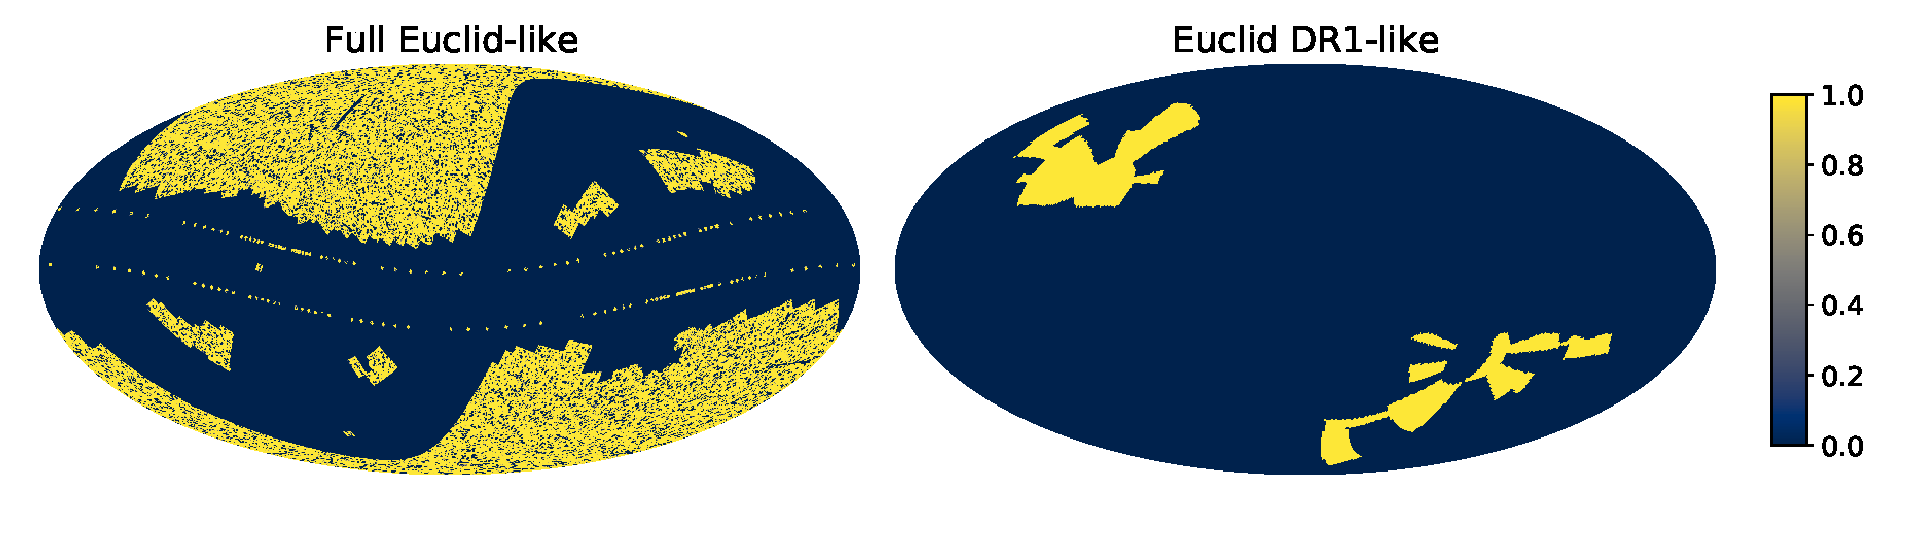
\includegraphics[width=\textwidth]{masks}
\caption{Full \Euclid{}-like and \Euclid{} DR1-like masks, which are used in Sections \ref{cov_sec:sims} and \ref{cov_sec:importance} to quantify the effects of different masks on the power spectrum covariance.}
\label{cov_fig:masks}
\end{figure}

For the theoretical covariance components described in \autoref{cov_sec:theory}, the same cosmology and redshift distribution as the simulations were used. A maximum multipole of $\ell_\text{max} = 8000$ was used in intermediate calculations to fully account for all relevant mode coupling, but the comparison was limited to $\ell \leq 3000$ because the $n_\text{side} = 4096$ maps that were used experience distortion from limited angular resolution above this point, as documented in \citet{Takahashi2017}. Higher resolution maps with $n_\text{side} = 8192$ are also available, so the $\ell$ range could in principle be extended, albeit with significantly increased computational requirements.

\subsubsection{Choice of redshift distribution}
\label{cov_sec:redshift}

The choice of redshift distribution used here---five Gaussian bins, centred on $z = 0.65$, 0.95, 1.25, 1.55, 1.85 with a standard deviation of 0.3---was made for simplicity,  with the relatively low number of redshift bins (five) also chosen for computational efficiency. Since there is freedom to enforce agreement between the redshift distributions in the simulations and theory, there is little additional value in choosing a more complicated, more realistic distribution. Future cosmological analyses of real \Euclid{} data are likely to use a larger number of bins with less overlap than is used here \citep[e.g.][]{Pocino2021}. There is no reason that this will affect the results presented in this chapter, although it should be noted that marginalising over nuisance parameters describing photometric redshift uncertainties will reduce the importance of all cosmological contributions to the covariance.

\subsection{Results}
\label{cov_sec:cov_vs_sims}

\autoref{cov_fig:cov_mats} shows correlation matrices for the simulated covariance compared to the total theoretical covariance for each mask, as well as the individual components of the theory covariance. There appears to be good agreement between the simulated and total theoretical correlation matrices for all three masks. The relative contributions from the three covariance components are discussed in \autoref{cov_sec:importance}.

\begin{figure}
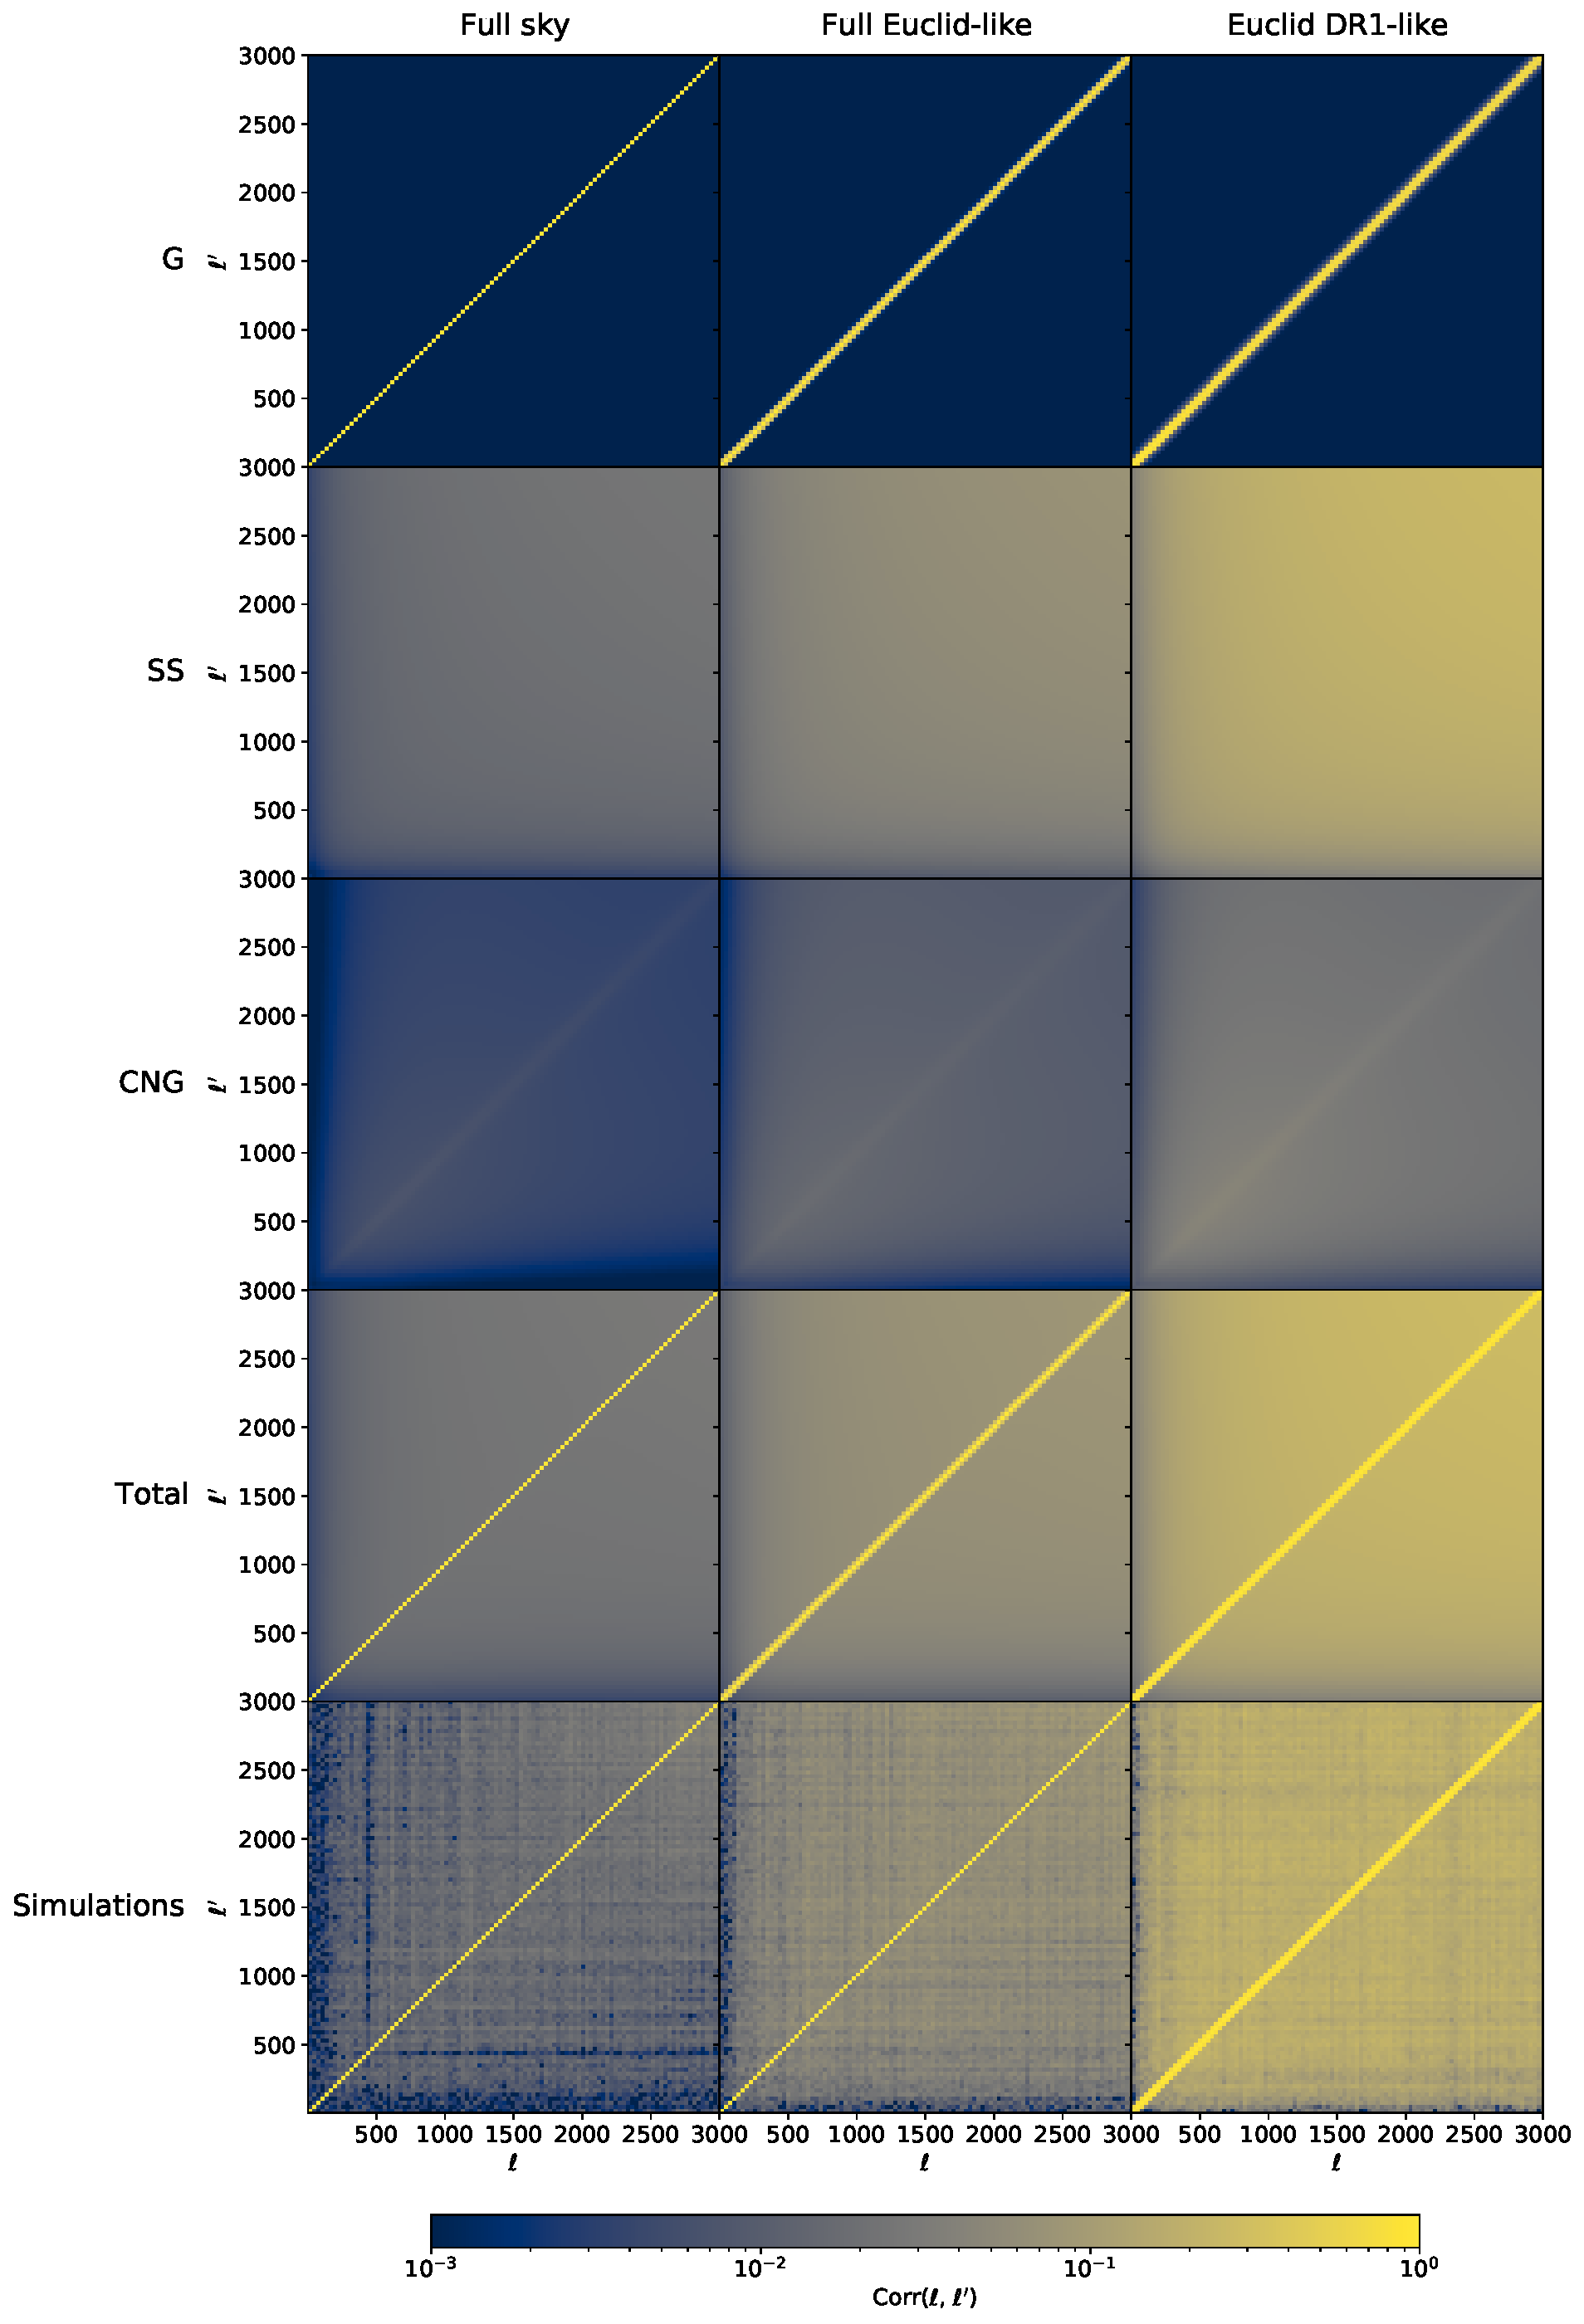
\includegraphics[width=.921\textwidth]{cov_mats} % so not too tall
\caption{Correlation matrices for the simulated covariance compared to the total theoretical covariance for each mask and for the individual components of the theory covariance: Gaussian (G), super-sample (SS), and connected non-Gaussian (CNG). The covariance shown here is for the shear $E$-mode power spectrum in the lowest redshift bin, without shape noise.}
\label{cov_fig:cov_mats}
\end{figure}

\autoref{cov_fig:cov_diags} shows a detailed comparison of certain diagonals of the covariance matrix. For the main diagonal ($\Delta \ell = 0$), the variance divided by the square of the power spectrum is shown, to remove any effects coming from disagreement in the power spectrum between the simulations and theory, which is not the focus of this work. For the off-diagonals ($\Delta \ell =$ 2, 10, 100) the correlation is shown.
In all panels the simulated line is a rolling average over 50 $\ell$s and the shaded region is the standard deviation over this range. For the full-sky and full \Euclid{}-like masks, excellent agreement is observed between the theory and simulations. For the more extreme \Euclid{} DR1-like mask there is a slightly worse, but still generally good, level of agreement. In particular, the super-sample covariance component is clearly correctly increasing with the severity of the sky cut to match the additional correlation found in the simulations. The relative sizes and importance of the three theory contributions are discussed further in \autoref{cov_sec:importance}.
We may conclude from Figures \ref{cov_fig:cov_mats} and \ref{cov_fig:cov_diags} that \texttt{CosmoLike}'s non-Gaussian covariance calculations appear to be suitably accurate, to the degree that can be assessed using these simulations.

\begin{figure}
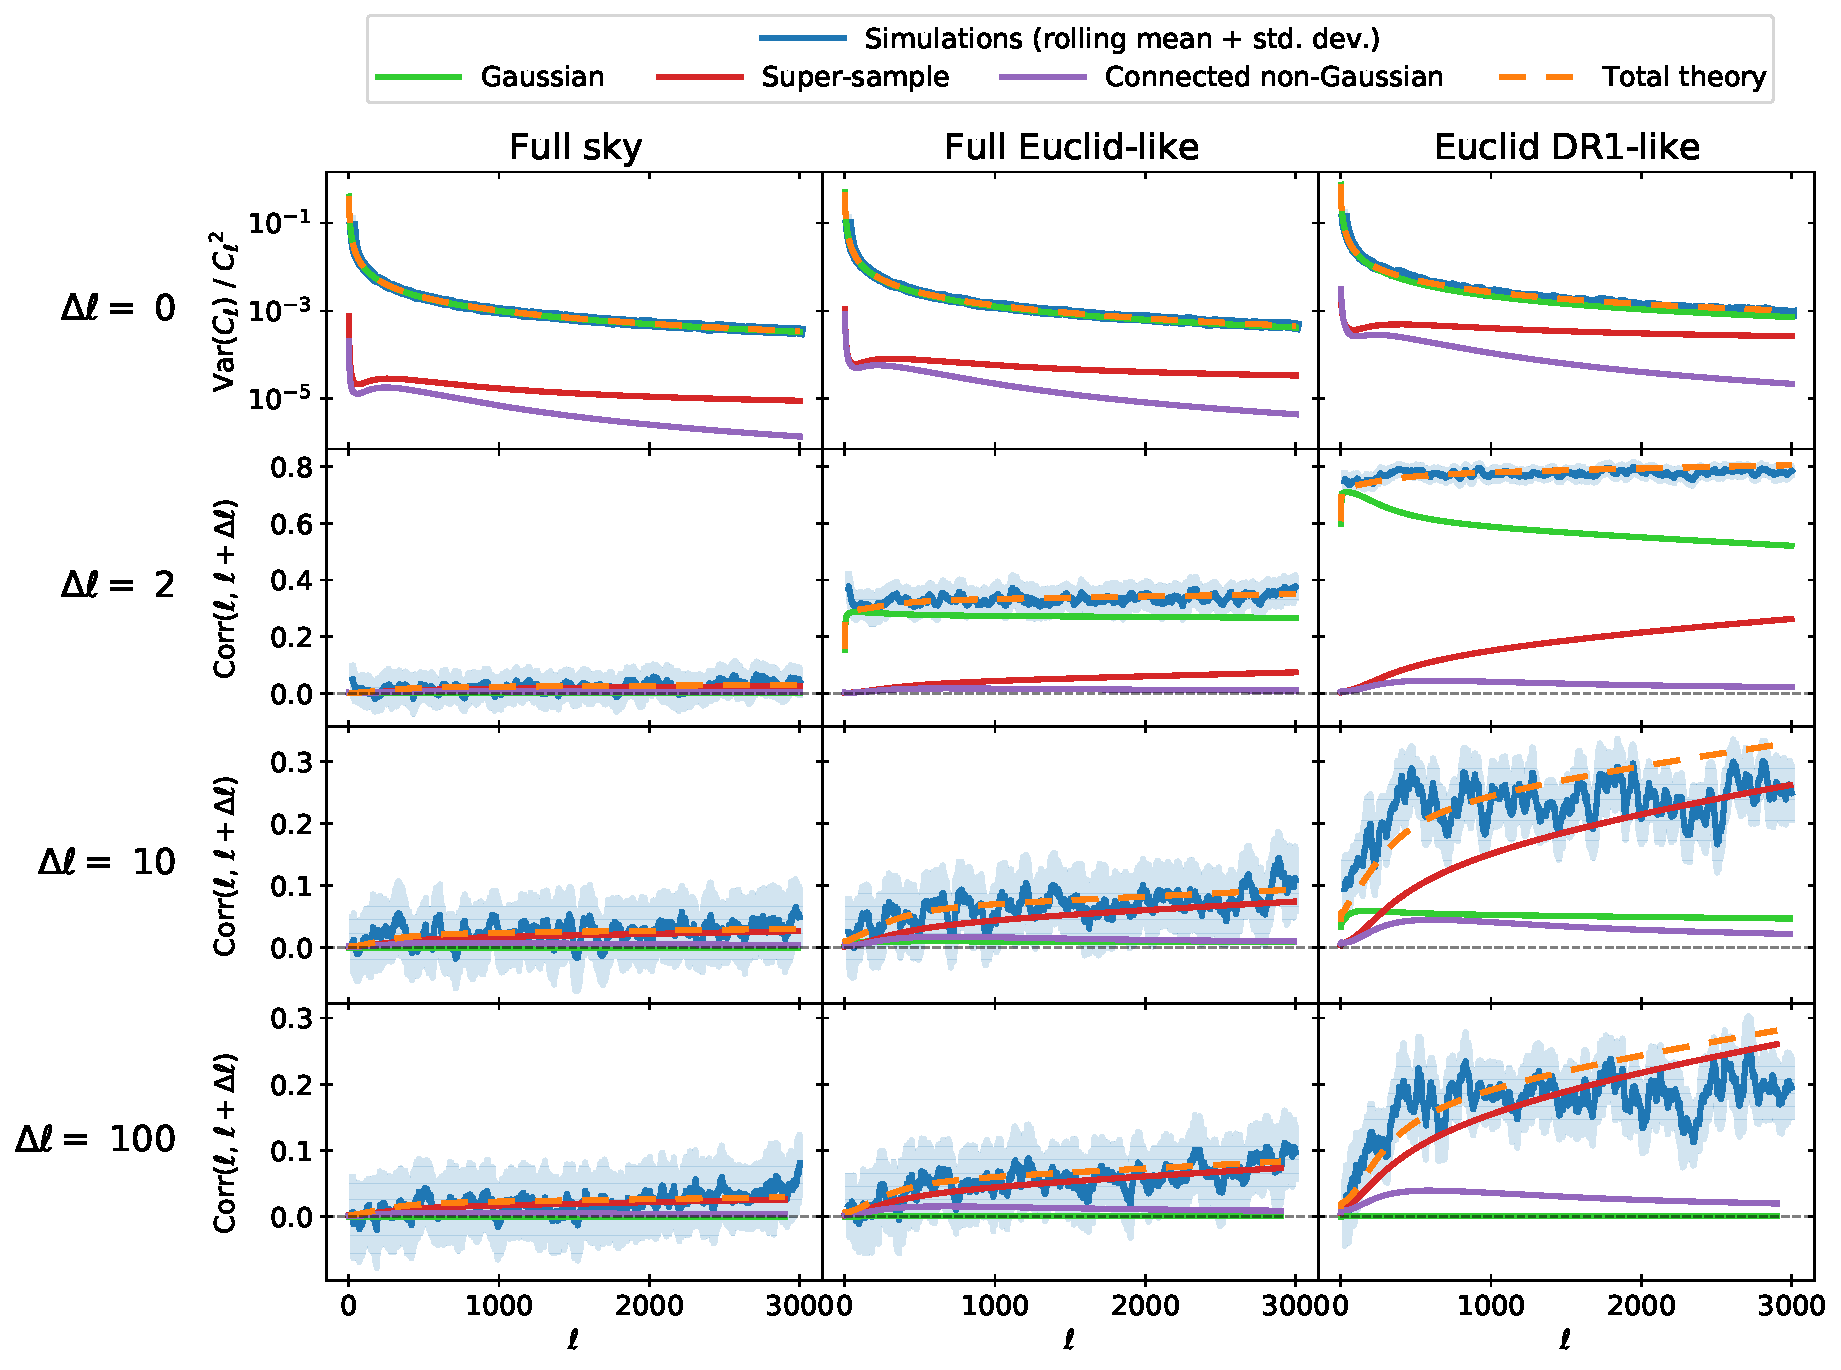
\includegraphics[width=\textwidth]{cov_diags}
\caption{Comparison between the covariance predicted by theory and measured from simulations, for the three masks. The top row shows the variance divided by the power spectrum squared, and the lower three rows show correlation. In all panels the simulated line is a rolling average over 50 $\ell$s, and the shaded region is the standard deviation over this range. The covariance shown here is for the shear $E$-mode power spectrum in the lowest redshift bin, without shape noise.}
\label{cov_fig:cov_diags}
\end{figure}

This comparison was also repeated for purely Gaussian fields, which were simulated using \texttt{healpy}.
The results are shown in \autoref{cov_fig:cov_diags_gauss}, where an excellent level of agreement is observed between the Gaussian field simulations and the prediction from the improved NKA, which is a significant improvement over the standard NKA (not shown).

\begin{figure}
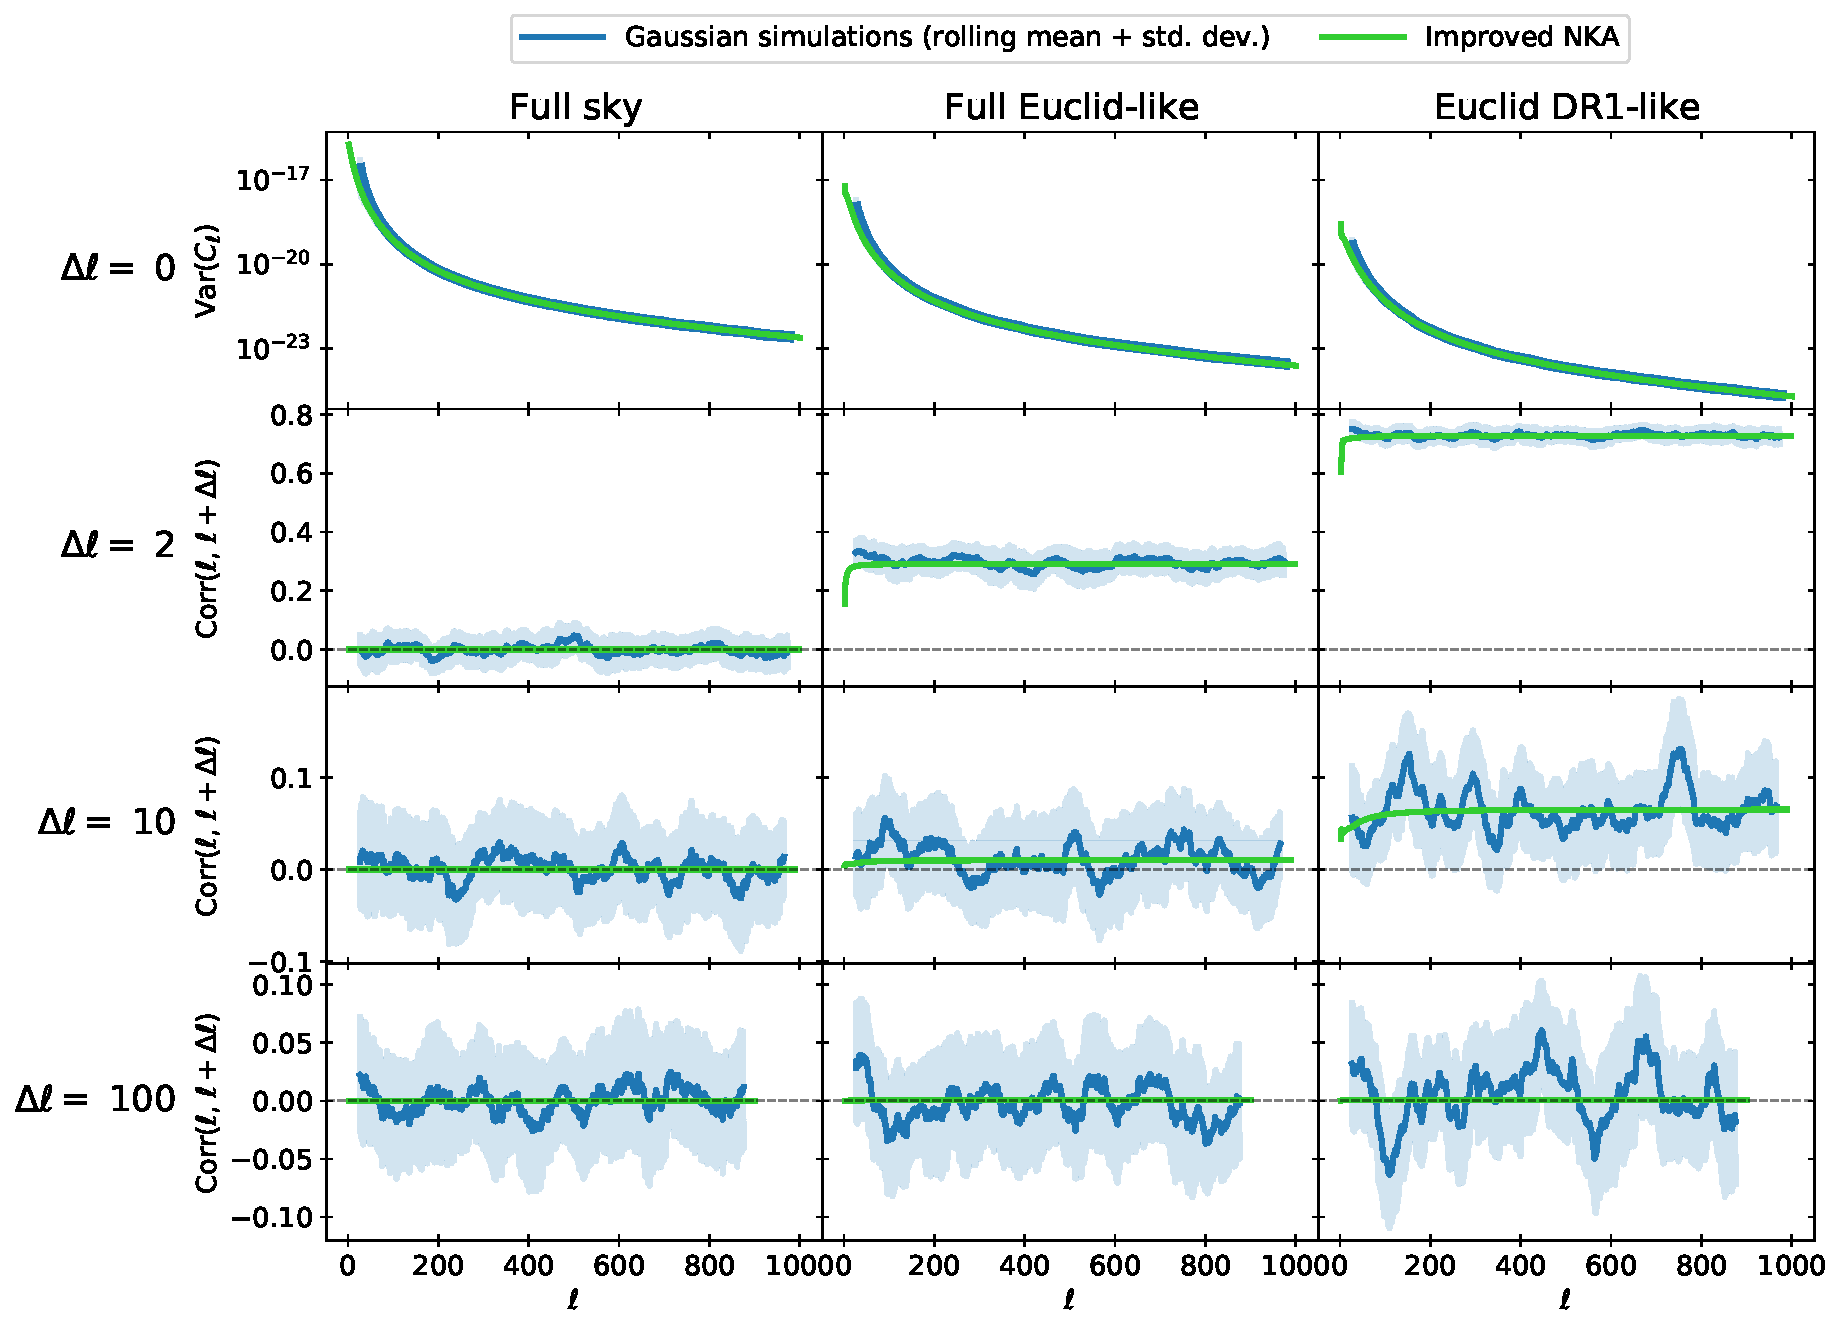
\includegraphics[width=\textwidth]{cov_diags_gauss}
\caption{Comparison between covariance measured from Gaussian field simulations and predicted using the improved NKA method, for the three masks. In all panels the simulated line is a rolling average over 50 $\ell$s, and the shaded region is the standard deviation over this range. No shape noise is included.}
\label{cov_fig:cov_diags_gauss}
\end{figure}

\section{Importance of covariance components and dependence on mask}
\label{cov_sec:importance}

This section addresses the size and importance of the different components of the cosmic shear pseudo-$C_\ell$ covariance, and how these properties depend on the mask.

\subsection{Relative sizes of components}
\label{cov_sec:rel_sizes}

\subsubsection{Without shape noise}

Let us first consider the case without shape noise, which has already been shown in Figures \ref{cov_fig:cov_mats} and \ref{cov_fig:cov_diags}.
It can be seen from the full correlation matrices plotted in \autoref{cov_fig:cov_mats} that the main diagonal of the matrix is dominated by the Gaussian component, which is purely diagonal in the full-sky case and visibly broadens slightly as the sky cut is increased. The super-sample covariance is the dominant off-diagonal component, particularly at higher $\ell$ but extending down visibly even to $\ell < 500$ in the case of the most extreme \Euclid{} DR1-like mask. The connected non-Gaussian contribution is barely visible on the colour scale, other than for the \Euclid{} DR1-like mask at low $\ell$.

A more detailed comparison of the relative sizes of the different components is possible with the selected diagonals shown in \autoref{cov_fig:cov_diags}. Again it is apparent that the main diagonal ($\Delta \ell = 0$) is dominated by the Gaussian component, but the extent to which this is the case is reduced as the sky cut is increased, as the contribution increases from both non-Gaussian components.
Moving away from the main diagonal, at $\Delta \ell = 2$ the Gaussian is still the largest component (except on the full sky, where its contribution is purely diagonal), but by $\Delta \ell = 10$ the super-sample component is dominant and increasing towards higher $\ell$.
It is clear that the super-sample covariance contribution increases with a more severe sky cut, though notably it is still visibly non-zero even for full-sky observations. The connected non-Gaussian component is the subdominant non-Gaussian contribution at all values of $\ell$ and $\Delta \ell$ for all masks.

\subsubsection{With shape noise}

\autoref{cov_fig:cov_diags_withnoise} shows an equivalent comparison of the sizes of the theoretical covariance components with shape noise included.
Gaussian shape noise is assumed, which---as introduced in \autoref{chap:est_like}---is included as a contribution to the power spectrum,
\begin{align}
C_\ell &\rightarrow C_\ell + N_\ell; \\
N_\ell &= \frac{{\sigma_\varepsilon}^2}{N_i},
\label{cov_eqn:nl}
\end{align}
where $\sigma_\varepsilon$ is the intrinsic galaxy shape dispersion per component and $N_i$ is the number of galaxies per steradian per redshift bin. A \Euclid{}-like galaxy number density of $30\,/\,\text{arcmin}^2$, equally split over five redshift bins, was assumed, along with a value of $\sigma_\varepsilon = 0.3$.

\begin{figure}
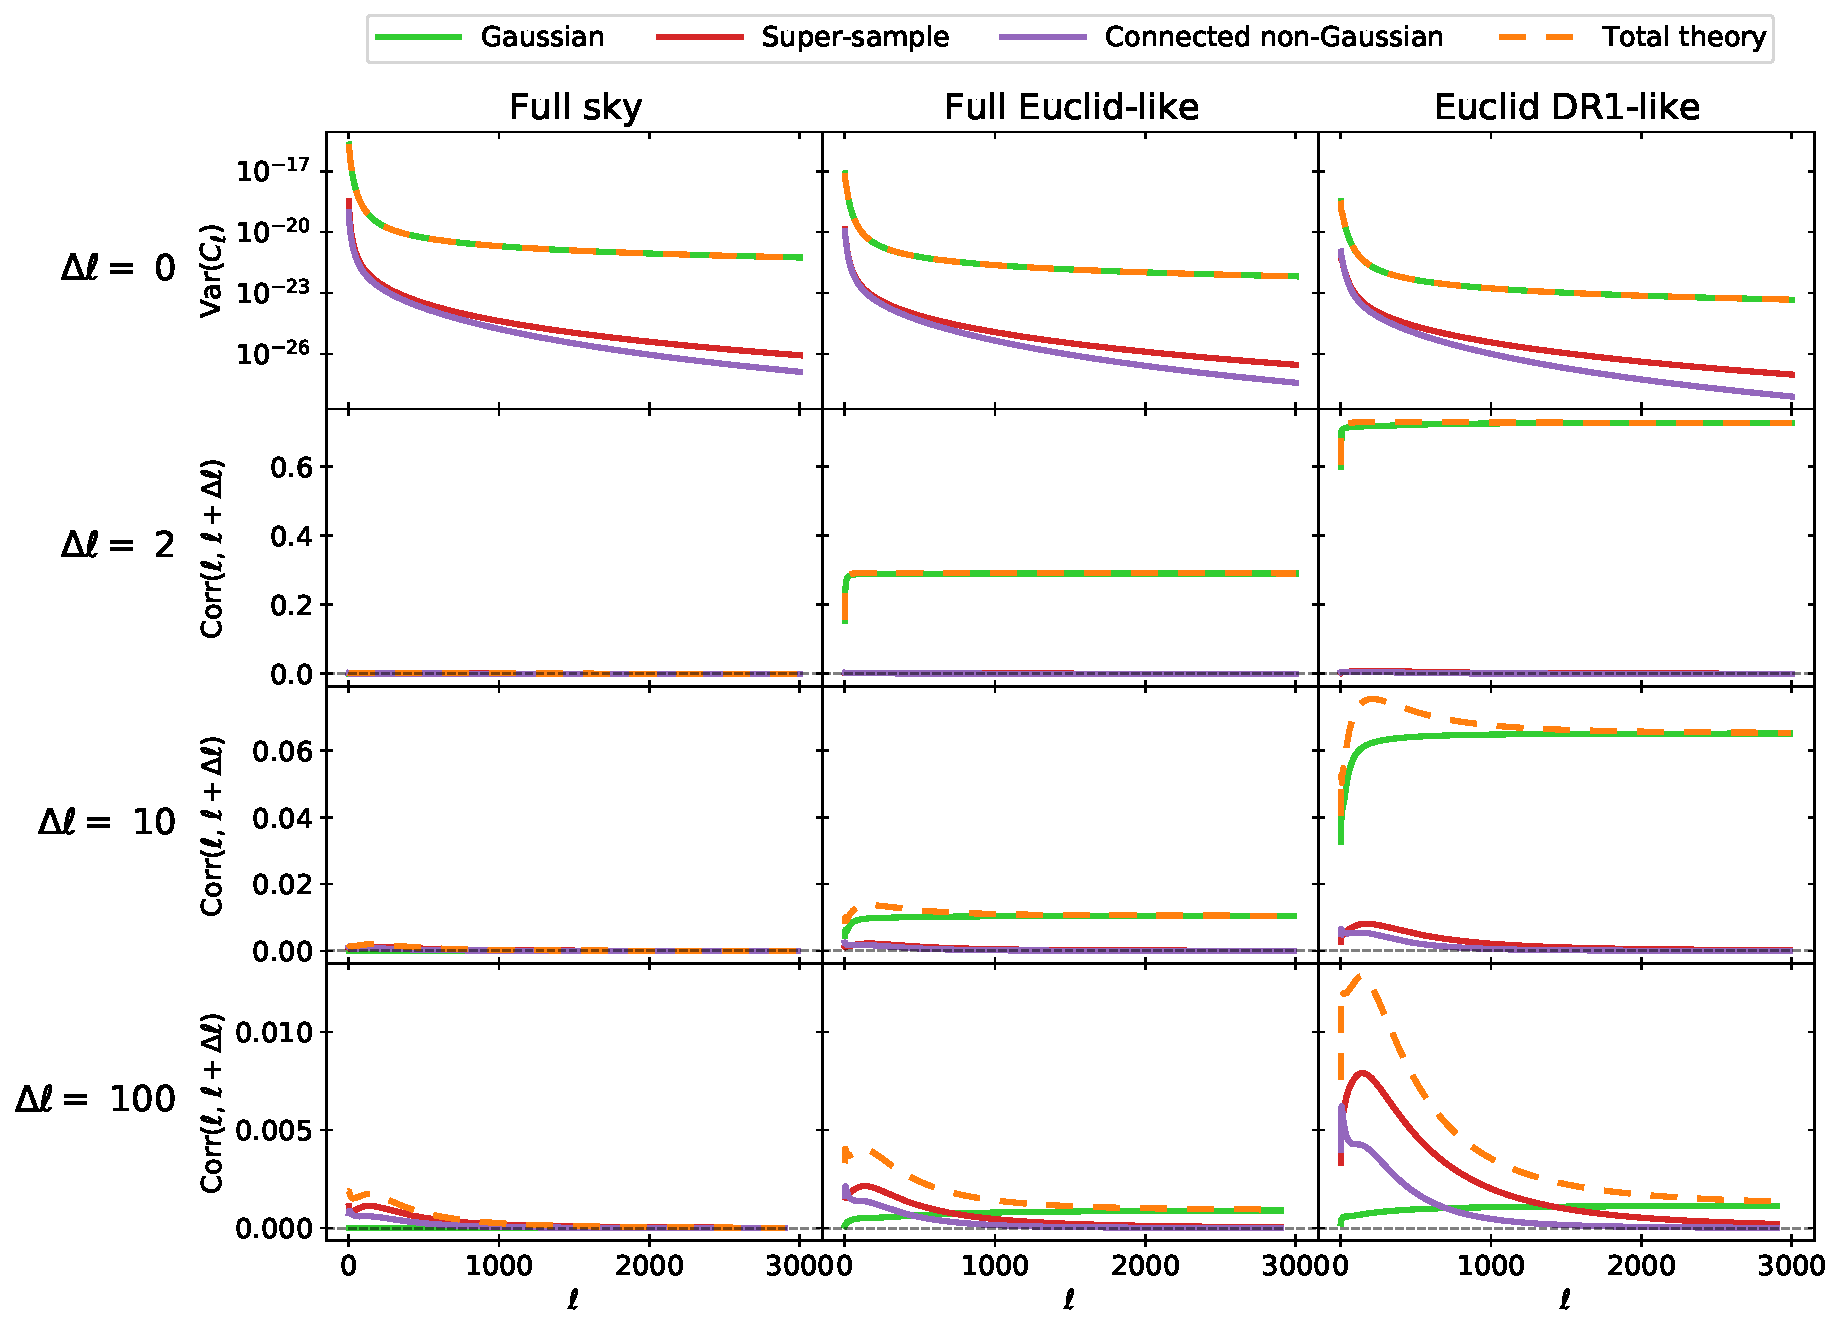
\includegraphics[width=\textwidth]{cov_diags_withnoise}
\caption{Comparison between contributions to the theoretical covariance for the three masks, with shape noise included
following Equation \eqref{cov_eqn:nl}. The top row shows the variance, and the lower three rows show correlation.}
\label{cov_fig:cov_diags_withnoise}
\end{figure}

With shape noise included, quite different behaviour to the no-noise case is found. The Gaussian-dominated main diagonal is substantially increased, especially at higher $\ell$, resulting in non-Gaussian off-diagonal correlations being significantly suppressed.
The result is that the Gaussian component is dominant at all $\ell$ as far away from the main diagonal as $\Delta \ell = 10$.
By $\Delta \ell = 100$, the Gaussian component is no longer dominant at lower $\ell$, but continues to account for the largest contribution at higher $\ell$: above $\ell \sim 1000$ for the full \Euclid{}-like mask and $\ell \sim 1500$ for the \Euclid{} DR1-like mask. This suggests that once shape noise is included, the Gaussian component is more important than the no-noise results in \autoref{cov_fig:cov_diags} suggest.

\subsection{Importance for parameter constraints}
\label{cov_sec:params}

While the relative size of the different covariance components studied in \autoref{cov_sec:rel_sizes} offers interesting insight into their behaviour, it says relatively little about the actual importance of each component. In particular, it is unclear to what extent the dominance of the Gaussian component on and close to the main diagonal is offset by its sub-dominance farther away from the main diagonal.
In this section, to gain more insight into this, mock parameter constraints are produced. Shape noise is included, following Equation \eqref{cov_eqn:nl}.

Here five redshift bins were used, including all auto- and cross-spectra ($E$-modes only), giving 15 power spectra in total.
Scales up to $\ell_\text{max} = 5000$ were included.
The full data vector for this setup would have $n =$ 75\,000 elements ($15 \times 5000$), which gives $n \left( n + 1 \right) / 2 =$ 2.8\,billion unique covariance elements. Due to the time needed to evaluate the projected matter trispectrum, it would be unfeasible to calculate the connected non-Gaussian contribution in full.
As a result, an angular binning approach was taken, with 12 logarithmically spaced bandpowers, and an approximation was used to obtain the connected non-Gaussian bandpower covariance from a more modest number of per-$\ell$ covariance calculations. This approximation is described and validated in \autoref{cov_sec:cng_approx}.
The Gaussian and super-sample covariance components were calculated in full, using scales up to $\ell_\text{max} = 8000$ for intermediate calculations, before being binned into bandpowers as
\begin{equation}
P_b = \sum_\ell \mathbfss{P}_{b \ell} C_\ell,
\label{cov_eqn:cl_to_bp}
\end{equation}
where $\mathbfss{P}$ is the bandpower binning matrix whose elements are given by
\begin{equation}
\mathbfss{P}_{b \ell} =
\begin{cases}
\dfrac{\ell \left( \ell + 1 \right)}{2 \pi}
\left[ \ell_\text{min}^{b + 1} - \ell_\text{min}^b \right]^{-1}
& \text{for } \ell_\text{min}^b \leq \ell < \ell_\text{min}^{b + 1}; \\
0 & \text{otherwise,}
\end{cases}
\label{cov_eqn:pbl}
\end{equation}
where $\ell_\text{min}^b$ is the lower edge of bin $b$.

A mock observation was obtained by sampling from a Gaussian likelihood with the total covariance. The input mean was the fiducial theory power spectra, plus noise for auto-spectra given by Equation \eqref{cov_eqn:nl}, mixed using the mixing matrix obtained using \texttt{NaMaster}, then binned following Equation \eqref{cov_eqn:cl_to_bp}. This random sampling process replicates the randomness of cosmic variance that is present in a real observation, and means that---as with real data---the resulting posterior distributions are not centred on the `true' input parameters.
Checks similar to those shown in \autoref{gl_Sec:nongauss_fields} confirmed that bandpowers measured from the \citet{Takahashi2017} simulations used in \autoref{cov_sec:sims} are no more non-Gaussian than those measured from Gaussian field simulations, and therefore since a Gaussian likelihood was shown to be sufficiently accurate for Gaussian fields in \autoref{chap:gauss_like}, it is a suitable choice here.

Parameter constraints were obtained by iterating over two-parameter grids produced using \texttt{CosmoSIS} \citep{Zuntz2015}, following the pipeline described in \autoref{gl_Sec:fs_method_theory}.\footnote{The pipeline includes the \texttt{CAMB} \citep{Lewis2000, Howlett2012} and \texttt{Halofit--} \texttt{Takahashi} \citep{Smith2003, Takahashi2012} modules.}
All other parameters were held fixed.
At each point in parameter space, theory bandpowers---calculated in the same way as the input mean to the observation described above---were compared to the observed bandpowers using a Gaussian likelihood with different combinations of covariance components.
All combinations necessarily include the Gaussian component, since this on its own is a valid positive definite covariance matrix, unlike the super-sample and connected non-Gaussian components.

\subsubsection{Connected non-Gaussian approximation}
\label{cov_sec:cng_approx}

As noted above, it is impractical to calculate the connected non-Gaussian component for all 2.8 billion unique elements of the full covariance matrix. Instead, an approximation was used to directly obtain its contribution to the bandpower covariance.
This approximation was designed to mimic two effects: the mixing of power by the survey mask, and the binning of individual multipoles into bandpowers. In this analysis, both of these processes are cosmology-independent: each shear field uses the same mask, and all power spectra use the same binning scheme. As a result, both processes should have approximately the same effect on every power spectrum, and consequently also every covariance block. Therefore, the approximation made here uses two sets of weights---one to mimic binning and the other to mimic mixing---which were calibrated for the covariance of the shear auto-power spectrum in the lowest redshift bin and then applied to all further blocks.

First, the connected non-Gaussian component was evaluated in full for a single covariance element per bandpower pair, for all combinations of power spectra. This was chosen to be for the weighted average $\ell$ in each bandpower, with the weights given by $\mathbfss{P}_{b \ell}$ (Equation \ref{cov_eqn:pbl}), rounded to the nearest integer. This vastly reduced the number of projected trispectrum calculations, to 16\,290.\footnote{This number comes from a reduced data vector of 12 bandpowers and 15 power spectra, giving a data vector of length $n = 12 \times 15 = 180$ and a number of unique covariance elements of $n \left( n + 1 \right) / 2 = 16\,290$.}
The result was then re-weighted using the weights calibrated using the covariance of the shear auto-power spectrum in the lowest redshift bin, which was calculated in full for the previous sections.

The weighting can be understood as a two-step process.
First, a `binning' weighting was applied, designed to mimic the effect of taking the full unbinned covariance matrix and binning it into bandpowers. Then a `mixing' weighting was applied, designed to mimic the effect of the mixing matrix. In both cases, the weights were obtained by carrying out the process in full for the shear auto-power spectrum in the lowest redshift bin.

This can be illustrated using equations as follows. For the first block (covariance of shear auto-power in the lowest redshift bin), the following procedure was used to transform the full unbinned covariance $\mathbfss{Cov}_\text{unbinned}$ into a final binned and mixed block $\mathbfss{Cov}_\text{mixed}$, via a binned and unmixed stage $\mathbfss{Cov}_\text{binned}$:
\begin{align}
\mathbfss{Cov}_\text{binned} &=
\mathbfss{P} ~ \mathbfss{Cov}_\text{unbinned} ~
\mathbfss{P}^\intercal; \\
\mathbfss{Cov}_\text{mixed} &=
\mathbfss{M} ~ \mathbfss{Cov}_\text{binned} ~
\mathbfss{M}^\intercal,
\end{align}
where $\mathbfss{P}$ and $\mathbfss{M}$ are the bandpower binning and pseudo-$C_\ell$ mixing matrices, respectively. Elements were selected from $\mathbfss{Cov}_\text{unbinned}$ corresponding to the weighted average $\ell$ within each bandpower to give $\mathbfss{Cov}_\text{sampled}$. The matrices of binning weights $\mathbfss{w}_\text{bin}$ and mixing weights $\mathbfss{w}_\text{mix}$ were then calculated as
\begin{align}
\mathbfss{w}_\text{bin} =
\frac{\mathbfss{Cov}_\text{binned}}
{\mathbfss{Cov}_\text{sampled}}
\qquad&\text{(elementwise);} \\
\mathbfss{w}_\text{mix} =
\frac{\mathbfss{Cov}_\text{mixed}}
{\mathbfss{Cov}_\text{binned}}
\qquad&\text{(elementwise).}
\end{align}
Finally, the sampled covariance blocks $\mathbfss{Cov}_\text{sampled}$ were calculated for every block in the full covariance matrix, and transformed to give approximate binned and mixed covariance blocks as
\begin{alignat}{2}
\mathbfss{Cov}_\text{binned\_approx} &=
\mathbfss{w}_\text{bin} *
\mathbfss{Cov}_\text{sampled}
\qquad&&
\text{(elementwise);} \\
\mathbfss{Cov}_\text{mixed\_approx} &=
\mathbfss{w}_\text{mix} *
\mathbfss{Cov}_\text{binned\_approx}
\qquad&&
\text{(elementwise).}
\end{alignat}
While this two-step weighting process could be equivalently formulated as a single step, separating the effect of the binning and mixing approximations allows for additional insight into their respective effects.

These approximations were validated by carrying out an equivalent process for the super-sample covariance matrix and comparing the results to those obtained using the full correct treatment.
Histograms of the ratios between the approximate and exact covariance for each step, for all elements of the bandpower covariance across all redshift bins, are shown in \autoref{cov_fig:cng_approx}.
Each step introduces a bias of order per cent on average (although conveniently in opposite directions) with a spread of a few per cent.
This is sufficiently accurate for the purposes of this work, especially considering that the connected non-Gaussian component is the smallest of the three, but nevertheless this small potential error should be borne in mind when interpreting the results. Since the super-sample and connected non-Gaussian covariance contributions were shown to be similarly smooth in \autoref{cov_sec:sims}, the fact that this approximation works well for the former suggests that it should too for the latter.

\begin{figure}
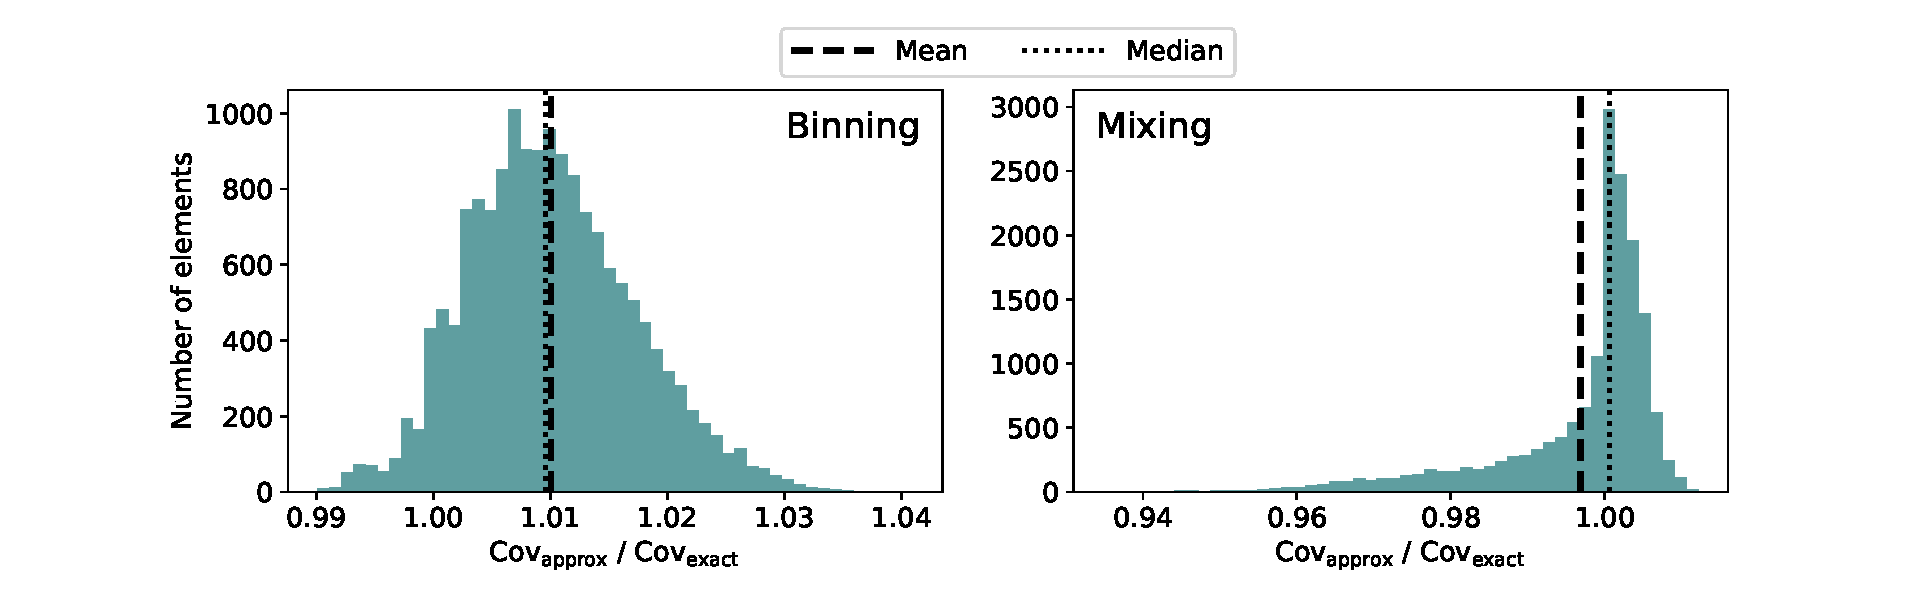
\includegraphics[width=\textwidth]{cng_approx}
\caption{Validation of the connected non-Gaussian approximation used to obtain the mock parameter constraints in \autoref{cov_sec:params}, which is described in \autoref{cov_sec:cng_approx}. Histograms of the ratio of the approximate to exact covariance are shown, for the `binning' (left) and `mixing' (right) steps, for all elements of the bandpower covariance matrix across all redshift bins, measured using the super-sample covariance. The results in all other sections are obtained using the connected non-Gaussian component calculated in full.}
\label{cov_fig:cng_approx}
\end{figure}

\subsubsection{Results}

Two-parameter constraints for different combinations of covariance components are shown in \autoref{cov_fig:2d_constraints}.
The top row shows dark energy equation of state parameters ($w_0$, $w_a$), where $w \left( a \right) = w_0 + w_a \left( 1 - a \right)$.
The bottom row shows the matter density $\Omega_\text{m}$ and the amplitude of the matter power spectrum at $z = 0$ on the scale of $8\,h^{-1}\,\text{Mpc}$, $\sigma_8$.
The three columns are for the three different masks. In each panel, all parameters other than the two shown are held fixed. Only the 1 and 3\,$\sigma$ credible regions are marked, which respectively contain the highest 68.3 and 99.7 per cent of the posterior probability mass. The relative areas of the $3\sigma$ credible region are listed for each combination of parameters and mask in \autoref{cov_tbl:rel_areas}.

\begin{figure}
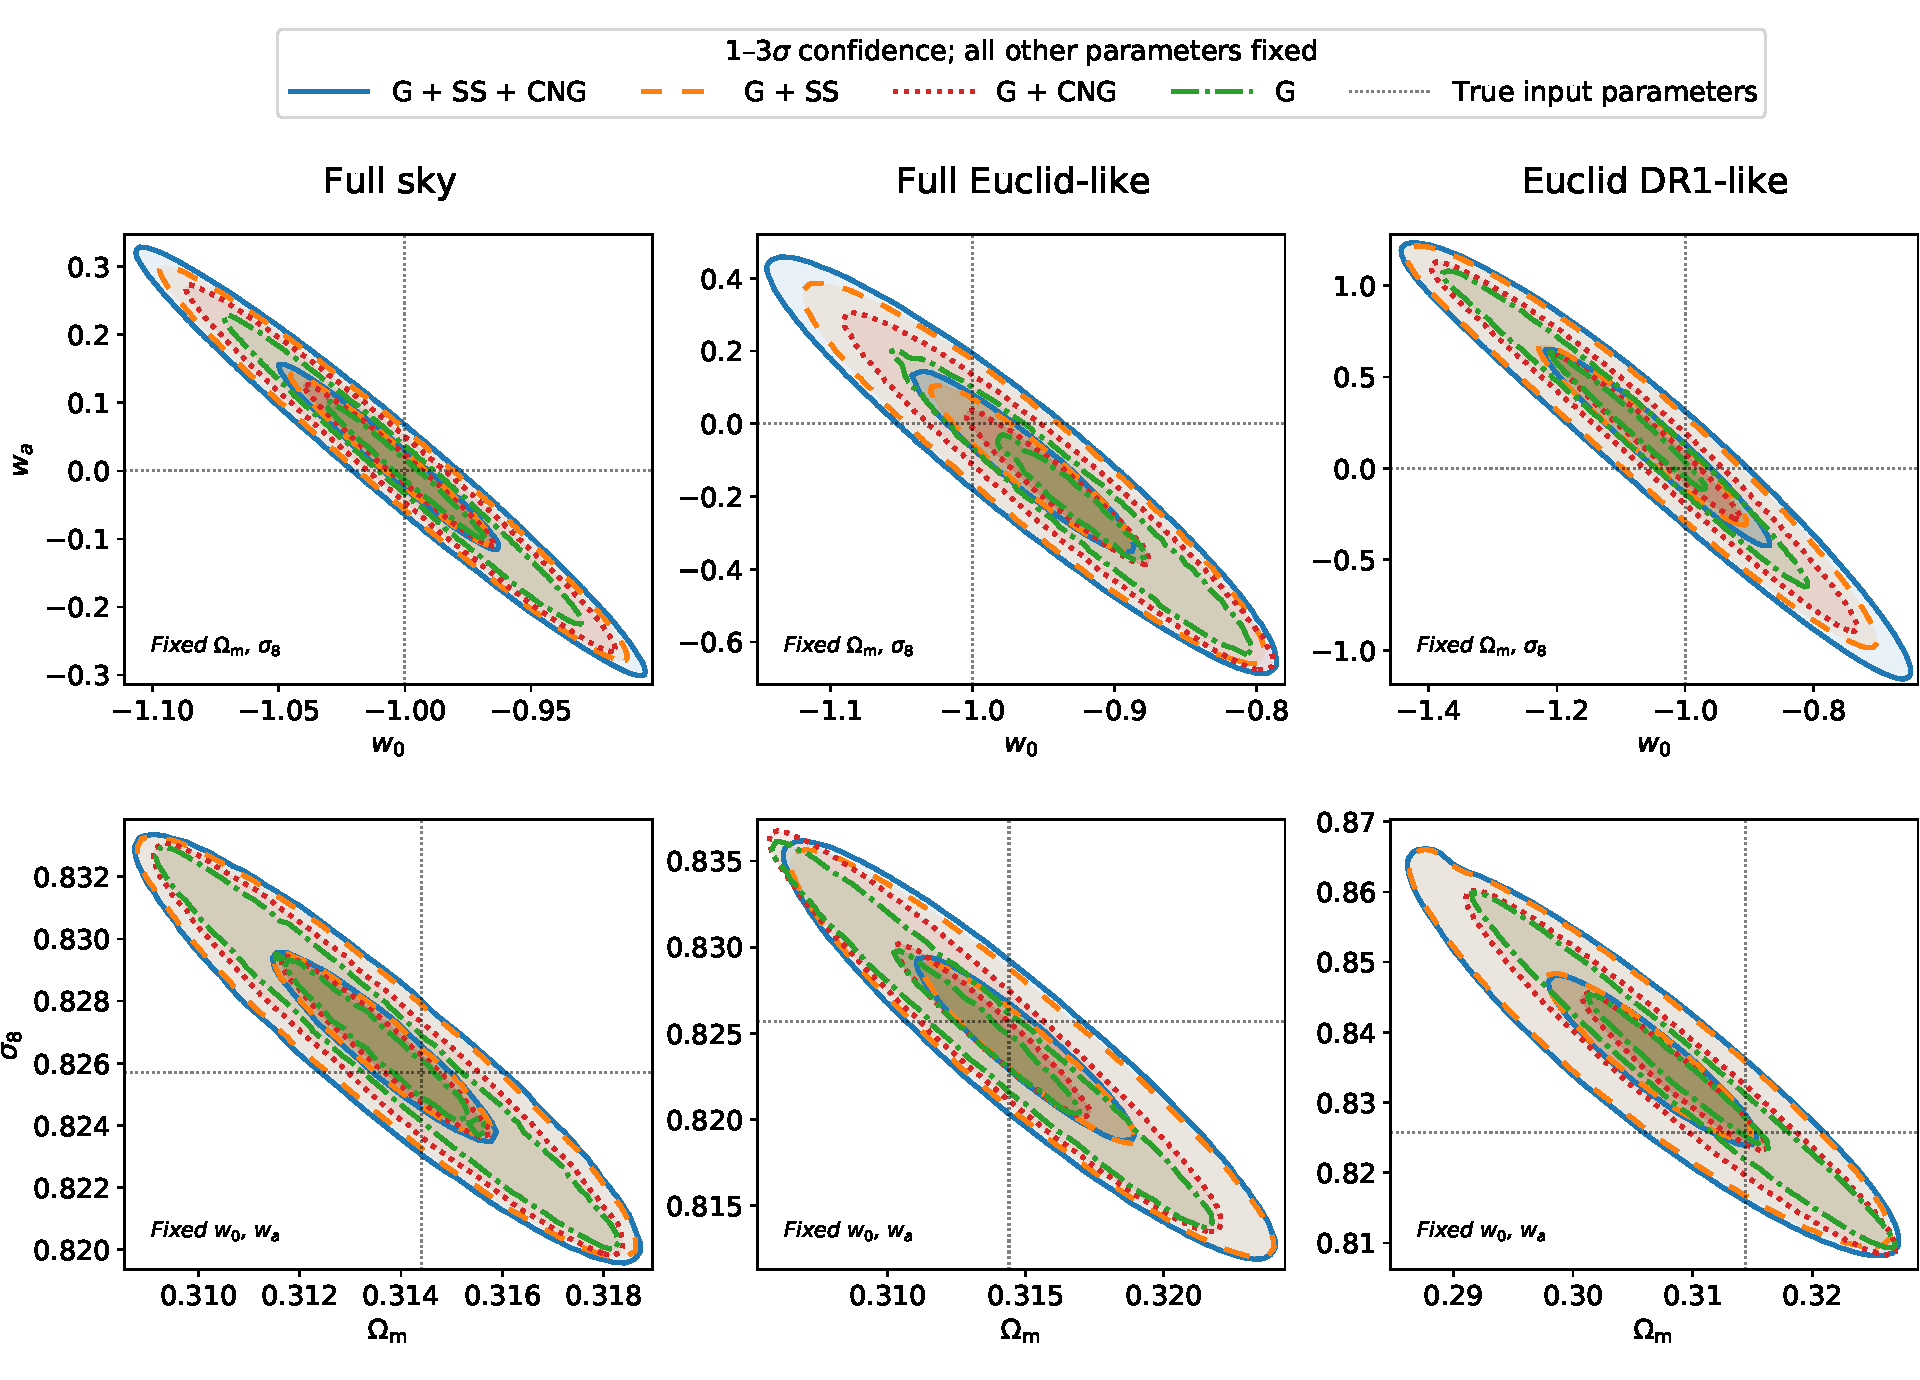
\includegraphics[width=\textwidth]{2d_constraints}
\caption{Two-parameter constraints for different masks and different combinations of covariance contributions: Gaussian (G), super-sample (SS), and connected non-Gaussian (CNG). Shape noise is included, following Equation \eqref{cov_eqn:nl}. In each panel, all parameters other than the two shown are held fixed. Only the 1 and 3\,$\sigma$ credible regions are marked, which respectively contain the highest 68.3 and 99.7 per cent of the posterior probability mass. The relative areas of each $3\sigma$ credible region are listed in \autoref{cov_tbl:rel_areas}. Note that the axis ranges differ between panels.}
\label{cov_fig:2d_constraints}
\end{figure}

\begin{table}[p]
{
\centering
\caption{Relative areas of $3\sigma$ credible regions in \autoref{cov_fig:2d_constraints}.}
\label{cov_tbl:rel_areas}
\vspace{.5em}
\bgroup
\def\arraystretch{1.3}
\begin{tabular}{llrrrr}
\hline
\multirow{2}{*}{Parameters} & \multirow{2}{*}{Mask} & \multicolumn{4}{c}{Relative area of $3\sigma$ credible region (\%)} \\
& & G + SS + CNG & G + SS & G + CNG & G \\ \hline \hline
\multirow{3}{*}{($w_0$, $w_a$)}
& Full sky & 100 & 82 & 63 & 38 \\
& Full \Euclid{}-like mask & 100 & 84 & 61 & 36 \\
& \Euclid{} DR1-like mask & 100 & 85 & 51 & 30 \\ \hline
\multirow{3}{*}{($\Omega_\text{m}$, $\sigma_8$)}
& Full sky & 100 & 90 & 70 & 49 \\
& Full \Euclid{}-like mask & 100 & 90 & 66 & 45 \\
& \Euclid{} DR1-like mask & 100 & 92 & 54 & 37 \\ \hline
\end{tabular}
\egroup

\vspace{1em}

}

{
% \small
% \textbf{Notes.}~
The table shows the relative area of the $3\sigma$ credible region in \autoref{cov_fig:2d_constraints} for each combination of parameters and mask and for different combinations of covariance components: Gaussian (G), super-sample (SS), and connected non-Gaussian (CNG). The relative $1\sigma$ areas are similar to the $3\sigma$ areas.
}
\end{table}

The Gaussian contribution (G) alone only covers 30--38 per cent of the full $3\sigma$ region for ($w_0$, $w_a$) and 37--49 per cent for ($\Omega_\text{m}$, $\sigma_8$). The Gaussian and connected non-Gaussian components combined (G + CNG) cover 51--63 and 54--70 per cent for ($w_0$, $w_a$) and ($\Omega_\text{m}$, $\sigma_8$), respectively, while the Gaussian and super-sample components combined (G + SS) cover 82--84 and 90--92 per cent. These results are broadly in line with the single-parameter error bar ratios obtained in \citet{Barreira2018b}.

There is some amount of apparent mask dependence: as the sky cut is increased, the relative area of G + SS sees a very small increase (by 2--3 per cent) whereas G + CNG and G see larger decreases (by 16--22 and 8--12 per cent, respectively). This is consistent with the expectation that super-sample covariance should become more important as the sky is cut further, since this excludes more modes from the survey.

There are also some small shifts in the posterior means between the different composite covariance results for a given mask, despite the fact that the mean of the Gaussian likelihood used in each case is identical and only the covariance differs. This demonstrates how an incorrect covariance leads to an incorrect weighting of the random scatter present in the data due to cosmic variance, and therefore to posterior constraints having not only the wrong size but an erroneous position too, although this is a small effect.

\subsubsection{Effect of marginalisation over additional parameters}

Motivation to explore the impact of marginalisation over additional parameters on the relative importance of each covariance component is provided by the results of \citet{Barreira2018b}. In that paper, the authors produced mock parameter constraints with different covariance contributions included, both for a single parameter at a time with all others fixed and for five parameters with all five allowed to vary simultaneously. For the latter case, they display marginalised two-parameter constraints \citep[their Figure 3]{Barreira2018b}. For ($w_0$, $w_a$) in particular (and to a lesser extent with some other parameter pairs), the $2\sigma$ credible region obtained with the Gaussian covariance alone appears roughly the same as that for the total covariance, to within the sampling noise. This is in contrast to their single-parameter constraints, for which the Gaussian covariance only produced $\sim$ 50 per cent of the $1\sigma$ uncertainty on $w_0$ obtained using the full covariance (see Figure 2 of \citealt{Barreira2018b}). This raises the question of whether marginalisation might reduce the differences between the constraints obtained using different combinations of covariance components.

Here, this question is investigated by performing a three-parameter likelihood analysis using the full \Euclid{}-like mask over ($w_0$, $w_a$, $\Omega_\text{m}$), with all other parameters still held fixed. One- and two-parameter marginalised constraints are shown in \autoref{cov_fig:3d_constraints}. \autoref{cov_tbl:marg} compares the relative areas and widths of one- and two-parameter $3\sigma$ credible regions before and after marginalisation over a third parameter.

\begin{figure} % [p]
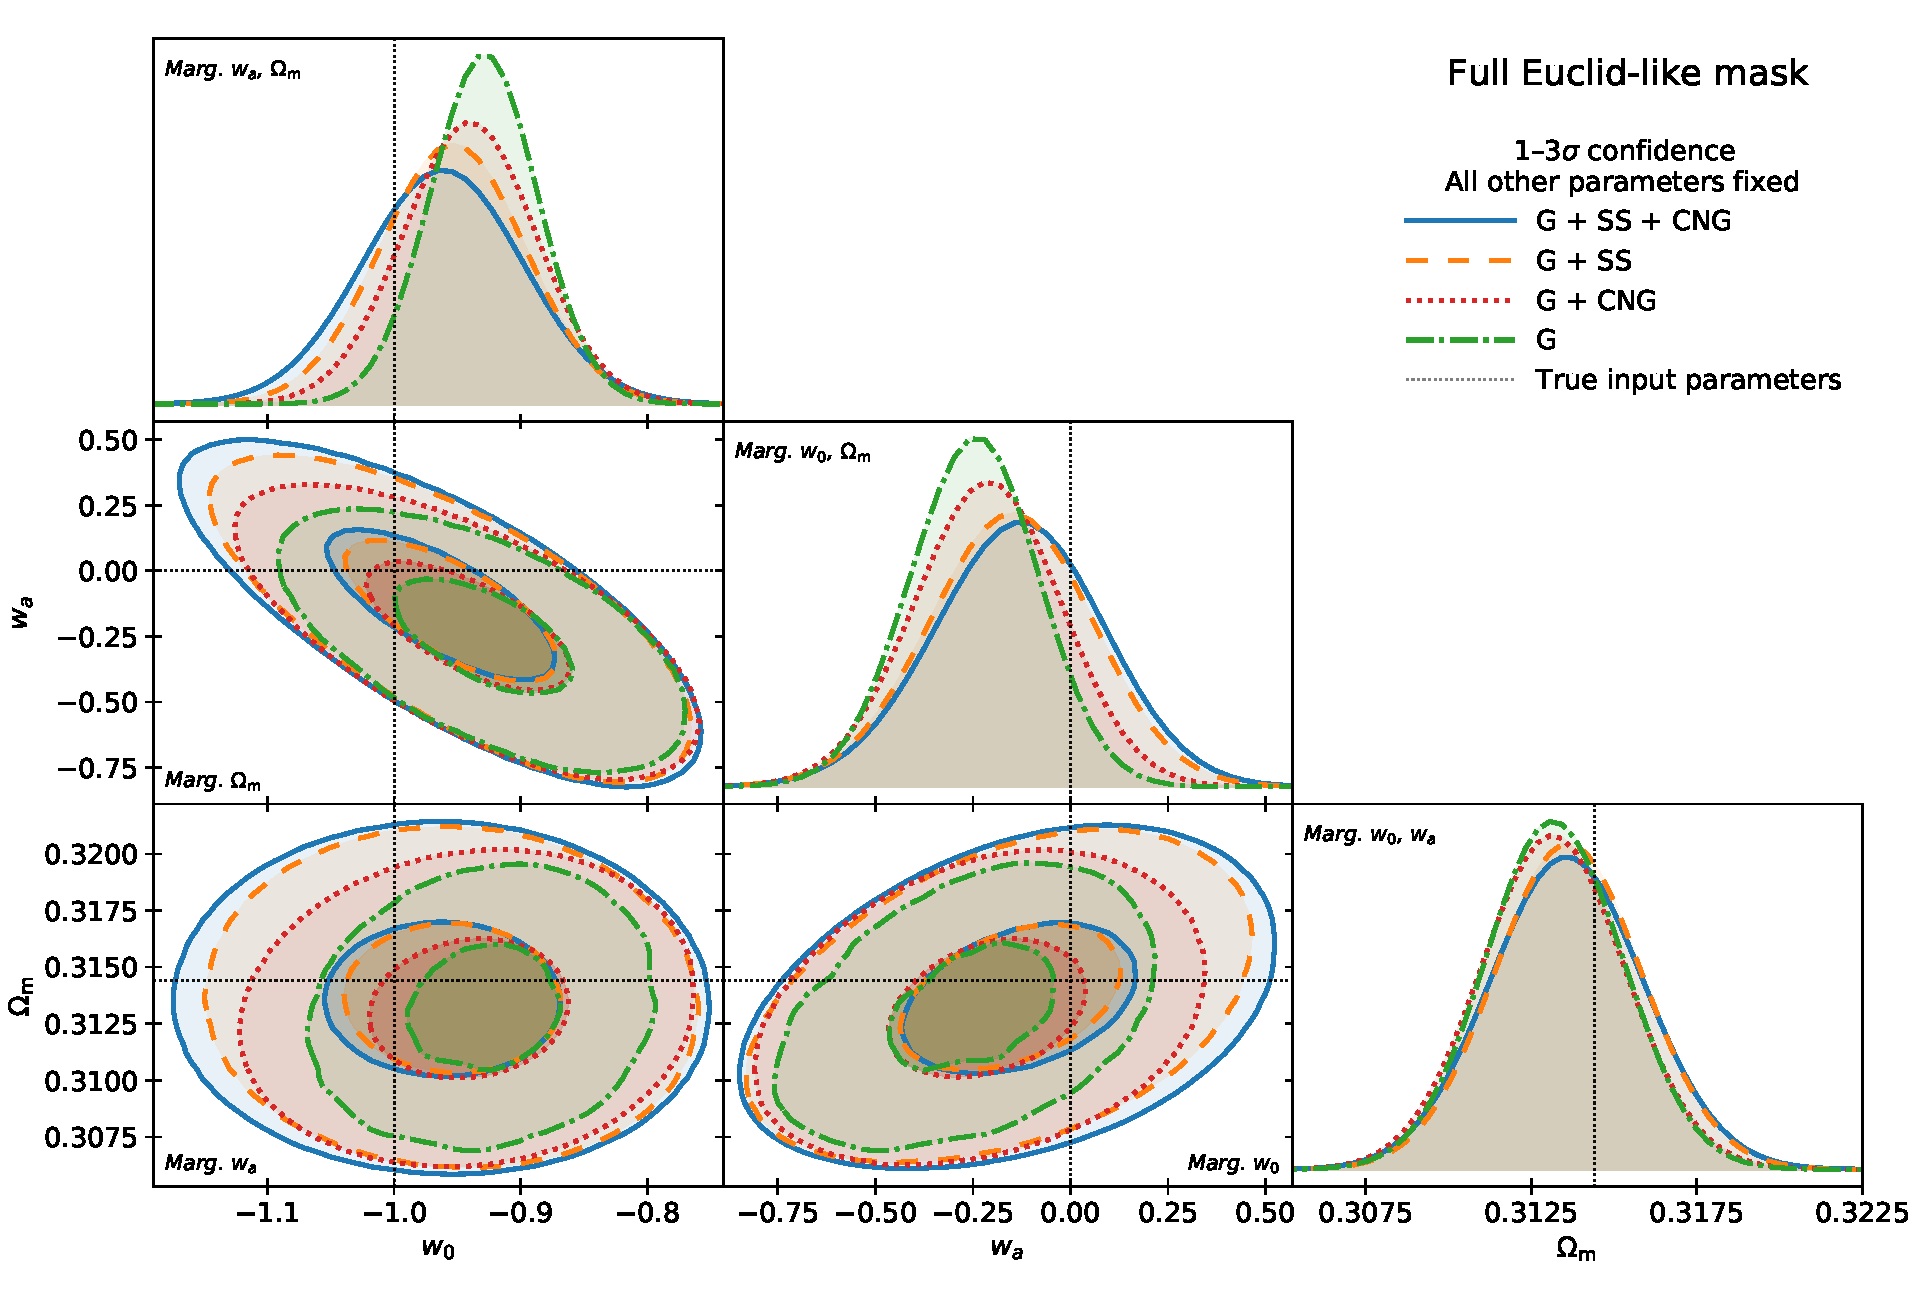
\includegraphics[width=\textwidth]{3d_constraints}
\caption{Two- and one-parameter marginalised constraints obtained from a joint three-parameter analysis of ($w_0$, $w_a$, $\Omega_\text{m}$) for the full \Euclid{}-like mask, including different combinations of covariance contributions: Gaussian (G), super-sample (SS), and connected non-Gaussian (CNG). Shape noise is included, following Equation \eqref{cov_eqn:nl}. The constraints in each panel have been obtained by marginalising over one or two parameters in the joint three-parameter posterior; for example, the panel marked `Marg. $w_a$, $\Omega_\text{m}$' has been marginalised over $w_a$ and $\Omega_\text{m}$. All other parameters are held fixed. Only the 1 and 3\,$\sigma$ credible regions are marked.}
\label{cov_fig:3d_constraints}
\end{figure}

While the relative areas in \autoref{cov_fig:3d_constraints} appear qualitatively similar to those in \autoref{cov_fig:2d_constraints}, there are in fact some substantial quantitative differences, as shown by the values in \autoref{cov_tbl:marg}. In particular, there is almost a doubling in the area of the constraints on ($w_0$, $w_a$) from the Gaussian covariance only (G) relative to the total covariance (G + SS + CNG)---from 36 to 69 per cent---when marginalising over $\Omega_\text{m}$ rather than holding it fixed. A similar but smaller increase is seen for the other subsets (G + SS, G + CNG) of the total covariance for the same parameters.

For constraints on $w_a$ alone, the width of the $3\sigma$ credible region for G relative to G + SS + CNG increases slightly when marginalising over both $w_0$ and $\Omega_\text{m}$ compared to only marginalising over $w_0$, and a similar slight increase is seen for G + SS and G + CNG. However, for constraints on $w_0$, there is a small decrease in relative widths when marginalising over both $w_a$ and $\Omega_\text{m}$ rather than only $w_a$. One reason for this difference in behaviour between $w_0$ and $w_a$ may be that---as seen in \autoref{cov_fig:3d_constraints}---there is clearly a much stronger correlation between $w_a$ and $\Omega_\text{m}$ than between $w_0$ and $\Omega_\text{m}$. Marginalisation over a strongly correlated parameter should broaden constraints more than marginalisation over a more weakly correlated parameter (indeed, marginalisation over a truly independent parameter should have no effect at all), but it is not obvious that this should change the ratio of relative areas rather than simply broadening all constraints by the same factor. Regardless of the origin of this behaviour, it does appear to be the case that marginalisation over additional parameters---particularly those with which the constrained parameters are correlated---affects the relative importance of the difference covariance contributions. This is in agreement with the findings of \citet{Barreira2018b}.

\begin{table}[t]
{
\centering
\caption{Impact of marginalisation on $3\sigma$ credible regions.}
\label{cov_tbl:marg}
\vspace{.5em}
\bgroup
\def\arraystretch{1.3}
\begin{tabular}{llrrrr}
\hline
\multirow{2}{*}{Parameter(s)} & \multirow{2}{*}{Marginalised over} & \multicolumn{4}{c}{Relative area or width of $3 \sigma$ credible region (\%)} \\
& & G + SS + CNG & \quad~ G + SS & \quad~ G + CNG & G \\ \hline\hline
\multirow{2}{*}{($w_0$, $w_a$)}
& --- & 100 & 84 & 61 & 36 \\
& $\Omega_\text{m}$ & 100 & 89 & 84 & 69 \\ \hline
\multirow{2}{*}{$w_0$}
& $w_a$ & 100 & 91 & 88 & 72 \\
& ($w_a$, $\Omega_\text{m}$) & 100 & 90 & 83 & 69 \\ \hline
\multirow{2}{*}{$w_a$}
& $w_0$ & 100 & 88 & 84 & 70 \\
& ($w_0$, $\Omega_\text{m}$) & 100 & 96 & 85 & 74 \\ \hline
\end{tabular}
\egroup

\vspace{1em}

}

{
% \small
The table shows the relative areas (for two-parameter constraints) and widths (for one-parameter constraints) of the $3\sigma$ credible regions obtained using different combinations of covariance contributions, Gaussian (G), super-sample (SS), and connected non-Gaussian (CNG), for the full \Euclid{}-like mask. Each row contains two sub-rows: the top sub-row is based on a two-parameter fit, which is marginalised over zero or one parameters; the bottom sub-row is based on a three-parameter fit, which is marginalised over one or two parameters. The relative $1\sigma$ areas are similar to the $3\sigma$ areas.
}
\end{table}

\section{Conclusions}
\label{cov_sec:conclusions}

As the era of next-generation weak lensing surveys such as \Euclid{} rapidly approaches, it is increasingly important to understand the properties of all steps of an analysis pipeline, including the covariance used in the likelihood.
\autoref{cov_sec:theory} has described how existing publicly available codes can be used in combination to calculate the full covariance matrix of cosmic shear pseudo-$C_\ell$ estimates, including the full details of an arbitrary mask.
It has been further shown in \autoref{cov_sec:sims} that existing simulations can be used to verify the accuracy of a theoretical covariance, which found a high degree of agreement and consistency between theory and simulations. This agreement persists for different masks, showing that the theoretical covariance contributions correctly account for both the cut-sky mode coupling that is inherent to the pseudo-$C_\ell$ method and the non-Gaussian mode coupling, including additional cut-sky super-sample covariance.

This is encouraging for the use of pseudo-$C_\ell$ estimators in weak lensing, whose convenience and speed make them an attractive choice of analysis framework for future surveys. However, an outstanding challenge with such estimators is the need to understand their statistical properties sufficiently well such that they can be used to deliver reliable cosmological constraints to the precision and accuracy needed by future high-precision weak lensing surveys. This challenge has now to a large degree been addressed since it is now known that not only is a Gaussian likelihood sufficient (\autoref{chap:gauss_like}), but a full covariance can be evaluated and validated using the methods shown in this chapter.

The results in this chapter have demonstrated that it is essential to include the non-Gaussian contributions to the covariance, even though cut-sky mode coupling means that the Gaussian covariance component dominates off-diagonal modes close to the main diagonal. The relative size and importance of the Gaussian component increases when including shape noise, but it has been shown in \autoref{cov_sec:importance} that only including the Gaussian component in parameter inference can lead to an underestimation of uncertainties by up to 70 per cent. The dominant non-Gaussian covariance component is the super-sample covariance, but neglecting the subdominant connected non-Gaussian covariance component can still lead to uncertainty underestimation on the scale of 10--20 per cent.
In addition, neglecting some covariance contributions can lead to biases in the position of posterior parameter constraints as well as their size.
However, a real cosmological analysis will require marginalisation over many nuisance parameters, which will decrease the relative importance of all cosmological contributions to the covariance, so these values should be taken as upper limits on the importance of each component.
Perhaps for this reason it was found in the analysis of DES Year 3 data in \citet{Friedrich2021} that the connected non-Gaussian contribution could be entirely neglected, but the results of this work suggest that this conclusion cannot be automatically extended to a \Euclid{}-like survey.
However, this need not be an inconvenience, since approximations of the kind described in \autoref{cov_sec:cng_approx} can be used to obtain the connected non-Gaussian component in a manageable amount of time with a loss of accuracy of only a few per cent on an already subdominant term. Finally, this chapter has shown that marginalisation over additional cosmological parameters may have a substantial effect on the relative importance of the different covariance components. We may conclude from this that it is important to take all marginalisation into account when, for example, determining the required accuracy of theoretical results for a particular science goal or producing forecasts of parameter constraints.
The consistency of these results with those of \citet{Barreira2018b} implies that cut-sky mode coupling has relatively little impact on the respective importance of the covariance components.

% % Uncomment to build alone without subfiles:
% \printbibliography[heading=bibintoc]
% \end{document}
